\documentclass{article}

\usepackage{amsmath}
\usepackage{amssymb}
\usepackage{enumerate}
\usepackage[spanish]{babel}
\usepackage{cancel}
\usepackage{caption}
\usepackage[margin=1.5in]{geometry}
\usepackage{graphicx}
\usepackage[utf8]{inputenc}
\usepackage{tcolorbox}
\usepackage{esint}
\usepackage{hyperref}
\hypersetup{
    colorlinks,
    citecolor=black,
    filecolor=black,
    linkcolor=black,
    urlcolor=black,
}

\renewcommand{\Bbb}{\mathbb}

\tcbuselibrary{theorems}

\title{Apuntes teórico-prácticos de Física I A (62.01) \\ Cátedra Menikheim \\ 1° C 2004}
\author{Darío Eduardo Ramos}

\definecolor{ududff}{rgb}{0.30196078431372547,0.30196078431372547,1}
\definecolor{cqcqcq}{rgb}{0.7529411764705882,0.7529411764705882,0.7529411764705882}

\begin{document}
\maketitle

\tableofcontents{}
\newpage

\section{Cinemática}

\subsection{Definiciones iniciales}

La \textbf{cinemática} es la rama de la física que describe el movimiento de los objetos sólidos sin considerar las causas que lo originan. 

El primer \textbf{modelo} que se adoptará para los cuerpos físicos a modelar será el de \textbf{punto material o partícula}: dichos cuerpos físicos serán considerados como sin volumen, pero sí con masa. Toda esa masa estará ``concentrada'' en el centro de masa del cuerpo, que será el punto que represente al objeto.

\textbf{Movimiento}: Un cuerpo será considerado en movimiento cuando cambie de posición a lo largo del tiempo respecto a un sistema de referencia considerado fijo o inercial. Más sobre esto último cuando se estudien los sistemas inerciales y no inerciales.

Cuando el cuerpo se desplaza desde una posición inicial dada por el vector $\overrightarrow{ r_i }$ a una posición final dada por el vector $\overrightarrow{ r_f }$, en un tiempo $\Delta t$, se definen las siguientes magnitudes vectoriales y escalares:

\begin{itemize}
\item \textbf{Vector desplazamiento:} $\overrightarrow{ \Delta r } = \overrightarrow{r_f} - \overrightarrow{r_i}$. Por como está definido, el vector $\overrightarrow{\Delta r}$ va de $\overrightarrow{r_i}$ hacia $\overrightarrow{r_f}$.
\item \textbf{Camino recorrido (escalar):}  $\Delta s$ = longitud del arco de trayectoria entre posición inicial y final.
\item \textbf{Vector velocidad media:} $\overrightarrow{v_m} = \frac{\overrightarrow{\Delta r}}{\Delta t}$
\item \textbf{Rapidez media (escalar):} $\overline{v} = \frac{\Delta s}{\Delta t}$
\item \textbf{Vector velocidad instantánea:}

\begin{equation}
\tcboxmath[colback=orange!25!white,colframe=orange]{
\overrightarrow{v} = \lim_{\Delta t \rightarrow 0} \frac{ \mathop{\overrightarrow{\Delta r}} }{\Delta t} = \frac{d\overrightarrow{r}}{\mathop{dt}}
}
\end{equation}

Nótese entonces que la velocidad instantánea es la derivada de la posición respecto al tiempo. Además, al ser $\overrightarrow{r}(t)$ una función vectorial del tiempo, $\overrightarrow{v}$ también lo es. Punto a punto, el vector $\overrightarrow{v}(t_0)$ es tangente a la curva de la trayectoria en el punto $\overrightarrow{r}(t_0)$ y su sentido es el del movimiento.
\item \textbf{Rapidez instantánea:}

\begin{equation}
v = \lim_{\Delta t \rightarrow 0} \frac{\Delta s}{\Delta t} = \frac{\mathop{ds}}{\mathop{dt}}
\end{equation}

\item \textbf{Vectores aceleración media e instantánea:}

\begin{equation}
\overrightarrow{a_m} = \frac{ \overrightarrow{ \Delta v } }{ \Delta t }
\end{equation}

\begin{equation}
\tcboxmath[colback=orange!25!white,colframe=orange]{
\overrightarrow{a} = \lim_{\Delta t \rightarrow 0} \frac{ \overrightarrow{ \Delta v } }{\Delta t} = \frac{ \mathop{d\overrightarrow{v}} }{ \mathop{dt} } = \frac{ \mathop{ d^2 \overrightarrow{r} } }{ \mathop{ dt^2 } }
}
\end{equation}

Cualquier cambio en el sentido, dirección o norma del vector velocidad indica que existe aceleración. Esto implica que en todo movimiento curvo hay aceleración no nula.

\end{itemize}

\subsection{Movimiento circular y movimiento curvo en general}

\subsubsection{Movimiento circular}

Algunas definiciones iniciales:

\begin{itemize}
\item \textbf{Velocidad angular (escalar):} $\omega = \frac{ \mathop{d\alpha} }{dt}$ = derivada del ángulo en función del tiempo.
\item \textbf{Ángulo en función del tiempo:} $\Delta \alpha = \omega \Delta t$
\item \textbf{Radianes:} $\alpha_{\mathop{rad}} = \frac{\text{longitud de arco}}{ \text{radio} }$
\item Relación entre $\omega$, el radio y la rapidez instantánea:

\begin{equation}
\alpha_{\mathop{rad}} = \frac{\text{longitud de arco}}{ \text{radio} } \Rightarrow \Delta \alpha = \frac{ \Delta s } {R} \Leftrightarrow \Delta s = \mathop{\Delta\alpha} \cdot R
\end{equation}

Reemplazando en la expresión general de la rapidez media:

\begin{equation}
\overline{v} = \frac{\Delta s}{\Delta t} \Rightarrow \overline{v} = \frac{\mathop{\Delta\alpha} \cdot R}{\Delta t} \Rightarrow v = \lim_{\Delta t \rightarrow 0} \underbrace{ \frac{\Delta \alpha}{\Delta t} }_{\omega} R \Rightarrow \tcboxmath[colback=orange!25!white,colframe=orange]
{ v = \omega R }
\end{equation}

De esta igualdad se puede concluir que si $\omega$ es constante, la rapidez instantánea también. Esto no aplica al vector velocidad, que tendrá norma constante, pero dirección variable.
\end{itemize}

\subsubsection{El vector velocidad}

Considerando $\overrightarrow{\omega}$ como un vector perpendicular, instante a instante, al plano del movimiento, se puede demostrar que para todo movimiento circular:

\begin{equation}
\tcboxmath[colback=orange!25!white,colframe=orange]{
\overrightarrow{v} = \overrightarrow{\omega} \times \overrightarrow{r}
}
\end{equation}

En esta igualdad, $\overrightarrow{r}$ es el vector posición. Dado que el sistema de referencia puede ser cartesiano o intrínseco, en ambos casos $\overrightarrow{r}$ se relaciona con el radio, aunque su expresión sea diferente.

Recuérdese que el vector resultado del producto vectorial es ortogonal a ambos vectores multiplicados a la vez. En este caso, $\overrightarrow{v}$ es ortogonal a $\overrightarrow{\omega}$ y también es ortogonal a $\overrightarrow{r}$. Además, el sentido de $\overrightarrow{v}$ está dado por la regla de la mano derecha.

\subsubsection{Coordenadas intrínsecas}

\begin{figure}[ht]
\centering
\caption{Coordenadas intrínsecas}
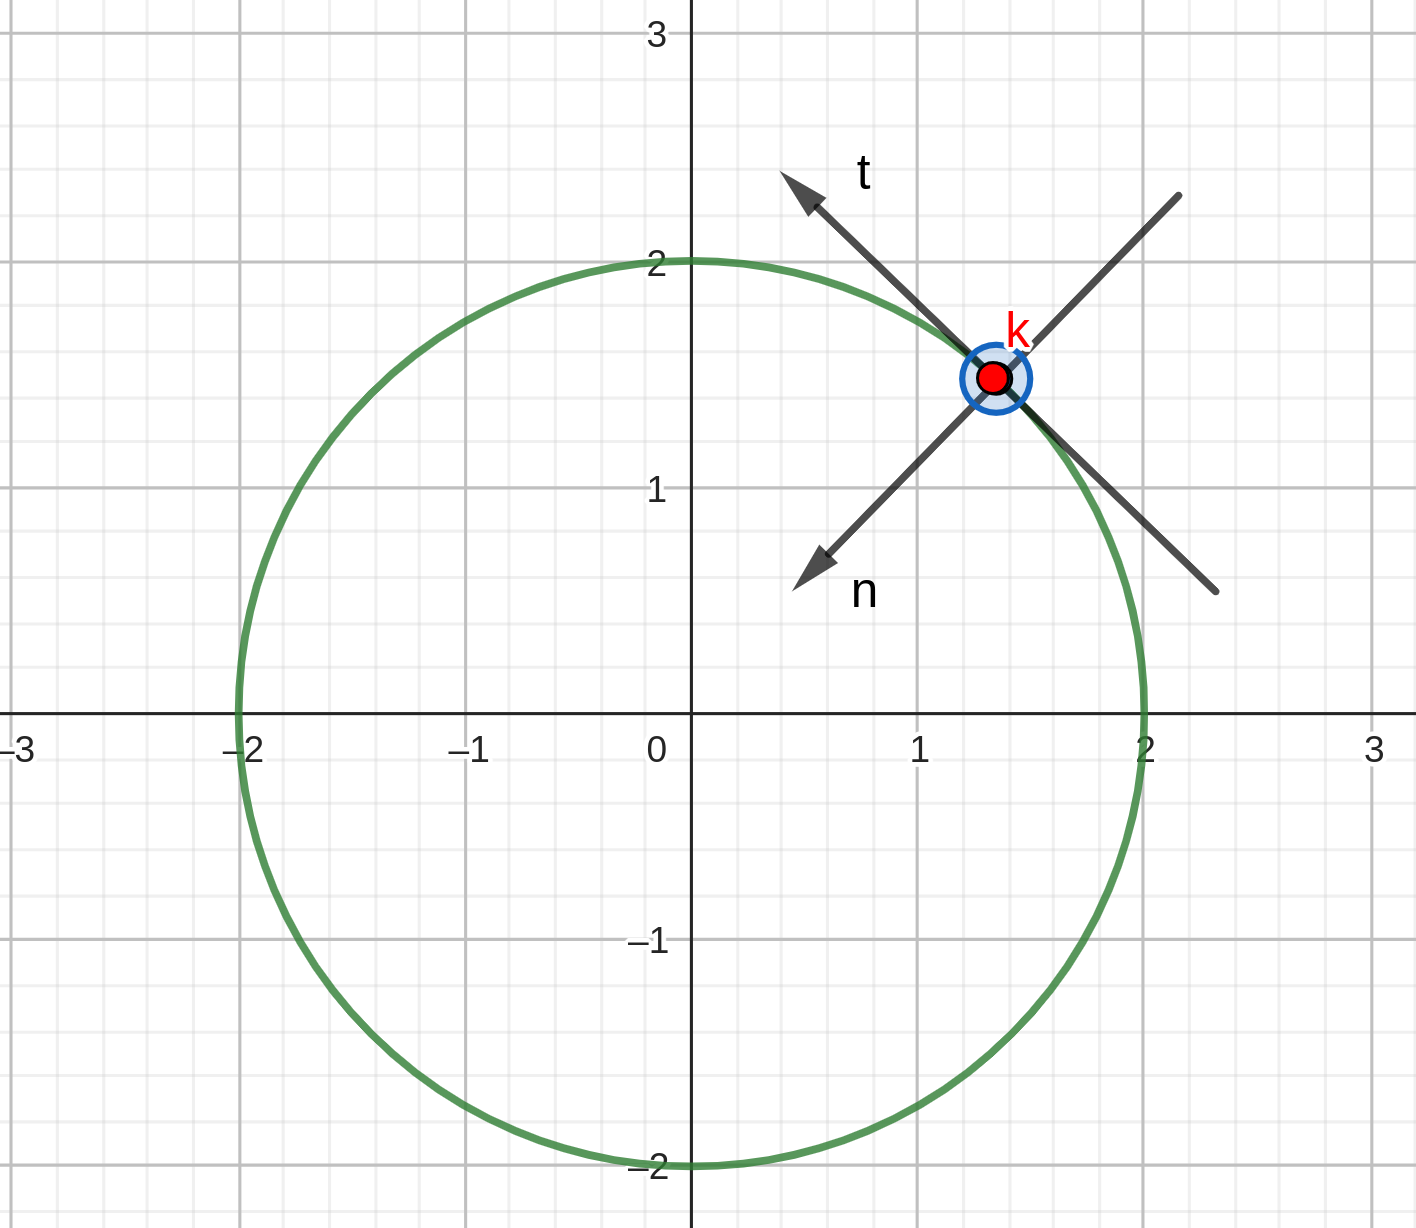
\includegraphics[scale=1]{../../common/img/62.01/theory/01-kinematics-intrinsic-coords.png}
\label{fig:intrinsicCoords}
\end{figure}

Obsérvese la figura \ref{fig:intrinsicCoords}. Para un instante determinado, el eje tangente $t$ se define positivo en el sentido de la velocidad. En cuanto al eje normal $n$, es positivo en el sentido de la concavidad, o sea hacia la parte interior del círculo. Finalmente, el eje binormal $k$, es positivo en el sentido de la aceleración angular $\gamma$. Es importante entender que este sistema de referencia es relativo a un instante específico de tiempo: para cada instante de tiempo, los ejes serán diferentes.

Con esta terna de ejes, resulta, si se denotan el radio del círculo con $R$, y los versores de los ejes con $\check{t}$, $\check{n}$ y $\check{k}$:

\begin{subequations}
\begin{align}
\overrightarrow{r} &= -R \check{n} \\
\overrightarrow{v} &= \omega R \check{t} \\
\overrightarrow{a_{\mathop{tg}}} &= \pm \gamma R \check{t} \\
\overrightarrow{a_{n}} &= \omega v \check{n}
\end{align}
\end{subequations}

Además, $R = ||\overrightarrow{r}||$ y $\gamma = ||\overrightarrow{\gamma}||$. Ahora bien, ¿de dónde salieron las expresiones de la aceleración tangencial y la aceleración normal? De derivar la velocidad. Ahora bien, al hacer eso, se utiliza el resultado de que la derivada de un producto vectorial sigue la misma regla que la derivada del producto de funciones. Verbigracia:

\begin{equation}
\overrightarrow{v} = \overrightarrow{\omega} \times \overrightarrow{r} \wedge \overrightarrow{a} = \frac{\mathop{d\overrightarrow{v}}}{\mathop{dt}} \Rightarrow \overrightarrow{a} = \underbrace{ \frac{\mathop{d\overrightarrow{\omega}}}{\mathop{dt}} }_{\overrightarrow{\gamma}} \times \overrightarrow{r} + \overrightarrow{\omega} \times \underbrace{ \frac{\mathop{d\overrightarrow{r}}}{\mathop{dt}} }_{\overrightarrow{v}}
\end{equation}

Resulta entonces:

\begin{equation}
\tcboxmath[colback=orange!25!white,colframe=orange, title=acelerac. en mov. circ.]{
\overrightarrow{a} = \underbrace{ \overrightarrow{\gamma} \times \overrightarrow{r} }_{\overrightarrow{a_{\mathop{tg}}}} + \underbrace{ \overrightarrow{\omega} \times \overrightarrow{v} }_{\overrightarrow{a_n}}
}
\end{equation}

En un movimiento circular, tanto $\overrightarrow{\omega}$ como $\overrightarrow{\gamma}$ jamás cambian su dirección, aunque sí puede cambiar su norma o su sentido.

Dado que $\overrightarrow{a_n}$ suele ser de especial interés por estar asociada a las fuerzas centrífugas, es de interés su norma:

\begin{equation}
a_n = ||\overrightarrow{a_n}|| = \omega v = \omega^2 R = \frac{v^2}{R}
\end{equation}

\subsubsection{Movimiento curvo generalizado}

Todo movimiento curvo puede ser analizado como la unión de movimiento circulares instantáneos, donde el radio es variable. Además, pasa a llamarse \textbf{radio de curvatura} y se denota con la letra $\rho$. Utilizando coordenadas intrínsecas, resulta:

\begin{equation}
\tcboxmath[colback=orange!25!white,colframe=orange]{
\overrightarrow{v} = \omega \rho \check{t}
}
\end{equation}

\begin{equation}
\tcboxmath[colback=orange!25!white,colframe=orange]{
\overrightarrow{a} = \underbrace{ \pm \gamma \rho \check{t} }_{\overrightarrow{a_{\mathop{tg}}}} + \underbrace{ \omega v \check{n} }_{\overrightarrow{a_n}}
}
\end{equation}

En este escenario generalizado, $\rho$ debe deducirse geométricamente, aunque esa no es la única forma de calcularlo. Por otro lado, puede decirse que $\overrightarrow{a_{\mathop{tg}}}$ está asociado a cambios en la norma de $\overrightarrow{v}$, en tanto $\overrightarrow{a_n}$ está asociado a cambios de dirección.

\subsection{Utilizando el cálculo integral}

Recordando que $\overrightarrow{v} = \frac{ \mathop{d \overrightarrow{r}} }{ \mathop{dt} }$ y $\overrightarrow{a} = \frac{ \mathop{d^2 \overrightarrow{r}} }{ \mathop{dt^2} }$, es posible utilizar el cálculo integral para hallar la magnitud original si se conoce su derivada. Esto ocurre siempre que dos magnitudes se relacionan a través de la derivada. Por ejemplo:

\begin{equation}
v_x = \frac{ \mathop{dx} }{ \mathop{dt} } \Rightarrow \mathop{ dx } = v_x \cdot \mathop{ dt } \Rightarrow \int_{x_0}^x \mathop{ dx } = \int_{t_0}^t v_x \cdot \mathop{ dt } \Rightarrow x - x_0 = \int_{t_0}^t v_x \cdot \mathop{ dt }
\end{equation}

Nótese que esto requiere conocer un punto de referencia $x_0 = r_x(t_0)$. Esta misma idea puede aplicarse para obtener la velocidad a partir de la aceleración.

\subsection{Calculando el radio de curvatura}

\begin{figure}[ht]
\centering
\caption{Radio de curvatura $\rho$}
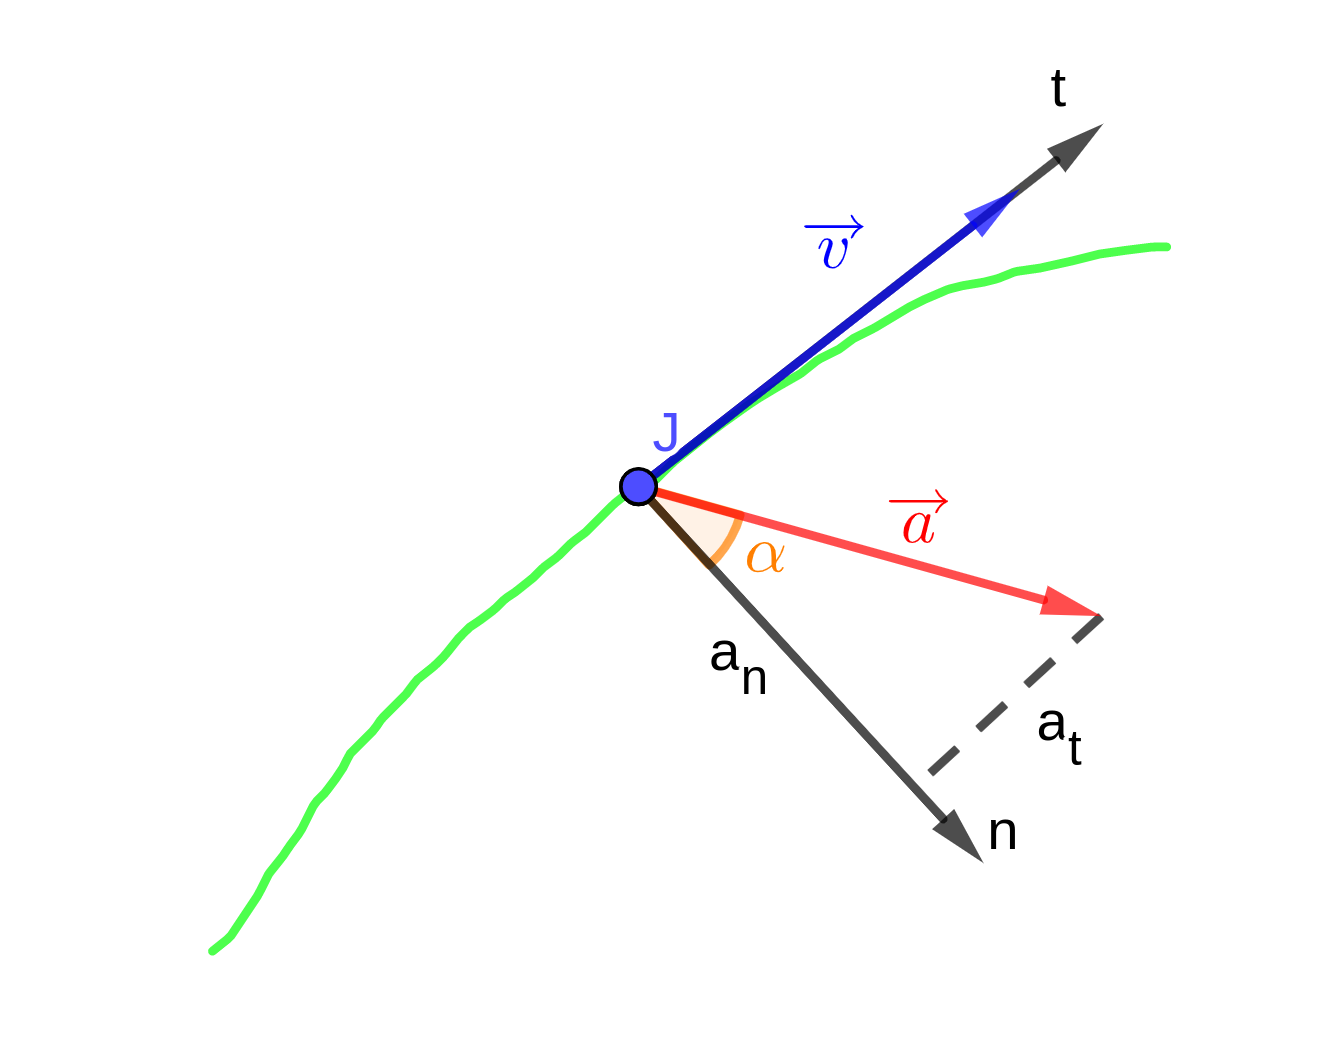
\includegraphics[scale=1.3]{../../common/img/62.01/theory/02-kinematics-rho.png}
\label{fig:rho}
\end{figure}

En base a la figura \ref{fig:rho}, dada la trayectoria, para calcular $\rho$ es necesario conocer la velocidad y la aceleración. Ello suele ser más directo utilizando un sistema de coordenadas intrínseco. En cuanto a $\alpha$, se deduce geométricamente. Con esos datos obtenidos, resulta:

\begin{subequations}
\begin{align}
a &= ||\overrightarrow{a}|| \\
a_n &= a \cos \alpha \wedge a_n = \frac{v^2}{\rho}
\end{align}
\end{subequations}

Finalmente:

\begin{equation}
\tcboxmath[colback=orange!25!white,colframe=orange]{
\rho = \frac{v^2}{a_n}
}
\end{equation}

\subsection{Movimiento relativo}

\subsubsection{Traslación}

\begin{figure}[ht]
\centering
\caption{Movimiento relativo - traslación}
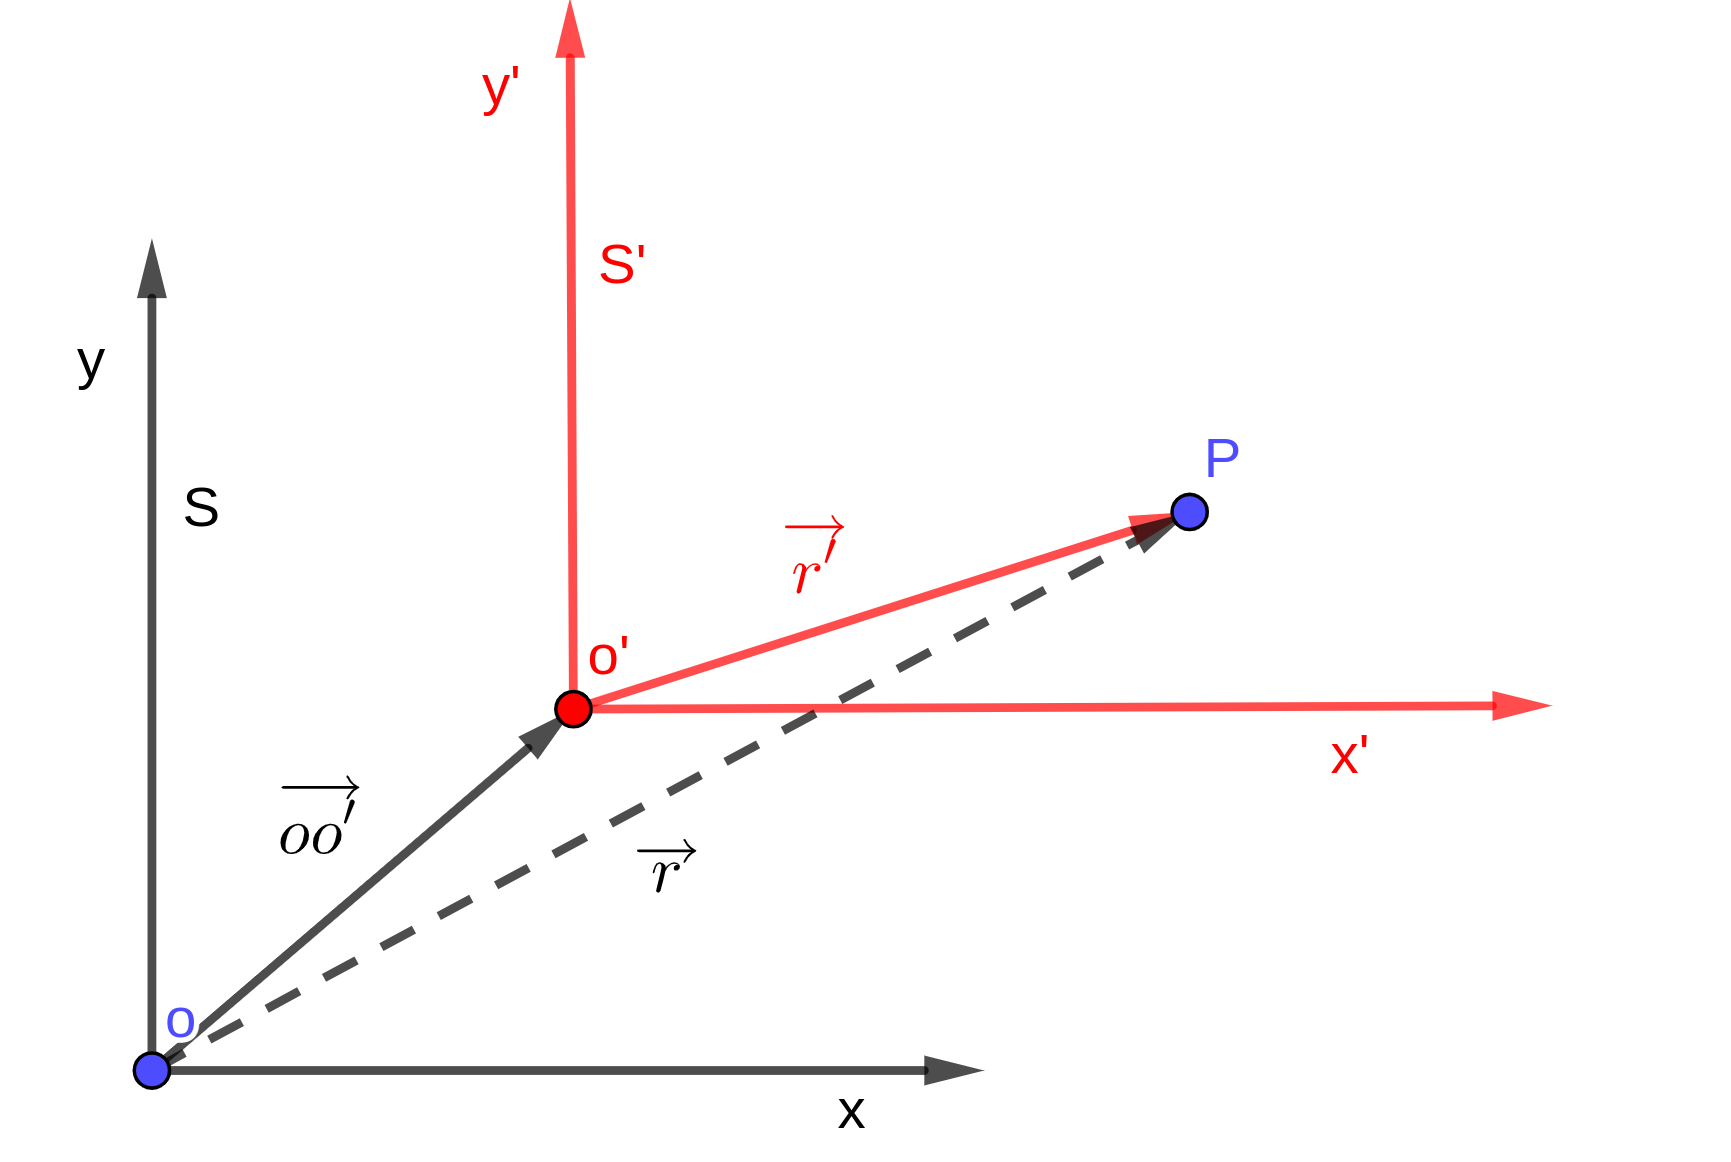
\includegraphics[scale=1.3]{../../common/img/62.01/theory/03-kinematics-rel-mov-tra.png}
\label{fig:relMovTra}
\end{figure}

En la figura \ref{fig:relMovTra}, se tiene un sistema de coordenadas $S$ que se considera fijo, y otro sistema $S'$ que se mueve respecto a $S$, pero sólo con traslación. Instante a instante, al no haber rotación, los ejes $x$ y $x'$ son paralelos en todo instante, al igual que $y$ e $y'$. Ello garantiza la siguiente igualdad vectorial, para todo tiempo $t$:

\begin{equation}
\overrightarrow{r} = \overrightarrow{oo'} + \overrightarrow{r'}
\end{equation}

\begin{itemize}
\item $\overrightarrow{r}$: Posición respecto al sistema fijo (posición absoluta).
\item $\overrightarrow{oo'}$: Posición del sistema móvil respecto al fijo (posición de arrastre). No perder de vista que esta magnitud también varía a lo largo del tiempo.
\item $\overrightarrow{r'}$: Posición respecto al sistema móvil (posición relativa).
\end{itemize}

Derivando miembro a miembro, resulta:

\begin{equation}
\tcboxmath[colback=orange!25!white,colframe=orange]{
\overrightarrow{v_{abs}} = \overrightarrow{v_{arr}} + \overrightarrow{v_{rel}}
}
\end{equation}

Derivando por segunda vez:

\begin{equation}
\tcboxmath[colback=orange!25!white,colframe=orange]{
\overrightarrow{a_{abs}} = \overrightarrow{a_{arr}} + \overrightarrow{a_{rel}}
}
\end{equation}

\subsubsection{Rotación}

\begin{figure}[ht]
\centering
\caption{Movimiento relativo - rotación}
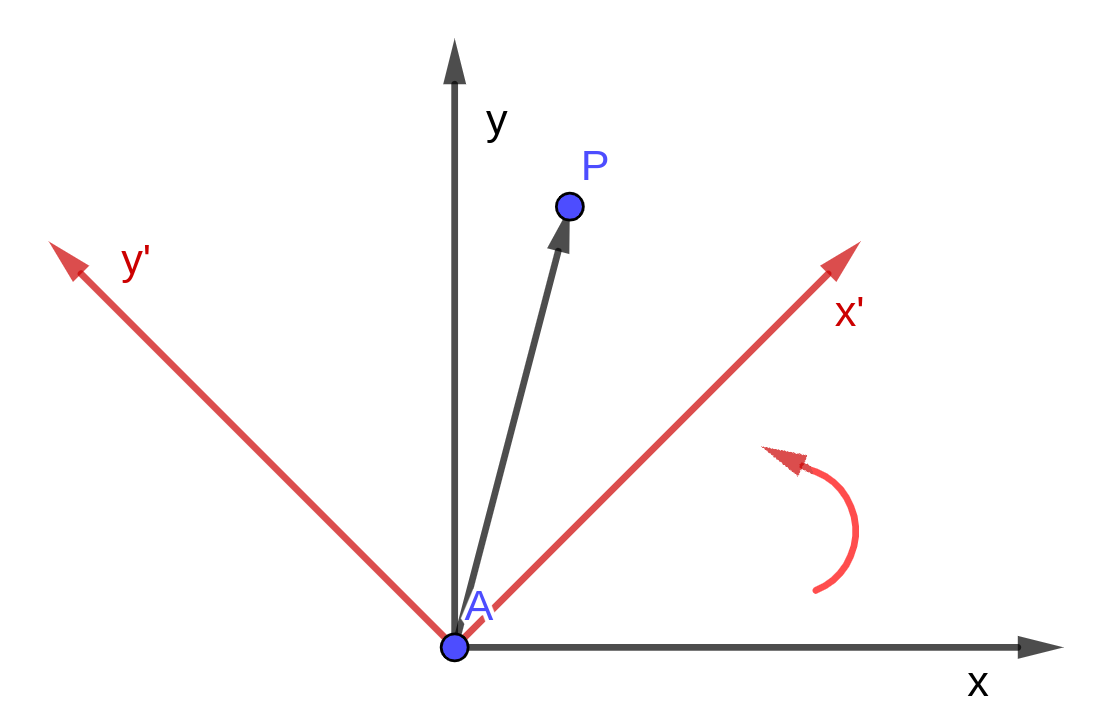
\includegraphics[scale=1.3]{../../common/img/62.01/theory/04-kinematics-rel-mov-rot.png}
\label{fig:relMovRot}
\end{figure}

En la figura \ref{fig:relMovRot}, el sistema $S'$ rota en sentido antihorario, sin transladarse, respecto al sistema $S$. Si se denota al versor $\check{i}$ como asociado al eje $x$, $\check{j}$ al eje $y$, y sus versiones primadas asociadas a los ejes de $S'$, es posible plantear:

\begin{subequations}
\begin{align}
\overrightarrow{r} &= x \check{i} + y \check{j} \\
\overrightarrow{r'} &= x' \check{i'} + y' \check{j'}
\end{align}
\end{subequations}

Derivando $\overrightarrow{r}$ respecto al tiempo, se obtiene $\overrightarrow{v_{abs}}$ de manera directa. Ahora bien, derivar $\overrightarrow{r'}$ no es tan directo, porque la posición de los versores primados varía a lo largo del tiempo. Aplicando la regla del producto, resulta:

\begin{equation}
\frac{ \mathop{ \overrightarrow{dr'} } }{ \mathop{dt} } = \frac{ \mathop{dx'} }{ \mathop{dt} } \check{i'} + x' \frac{ \mathop{d\check{i}'} }{ \mathop{dt} } + \frac{ \mathop{dy'} }{ \mathop{dt} } \check{j'} + y' \frac{ \mathop{d\check{j}'} }{ \mathop{dt} }
\end{equation}

Para analizar qué son las derivadas de los versores, considérese la variación de posición de uno de ellos a lo largo del tiempo, entre dos instantes.

\begin{figure}[ht]
\centering
\caption{Movimiento relativo - rotación - versores}
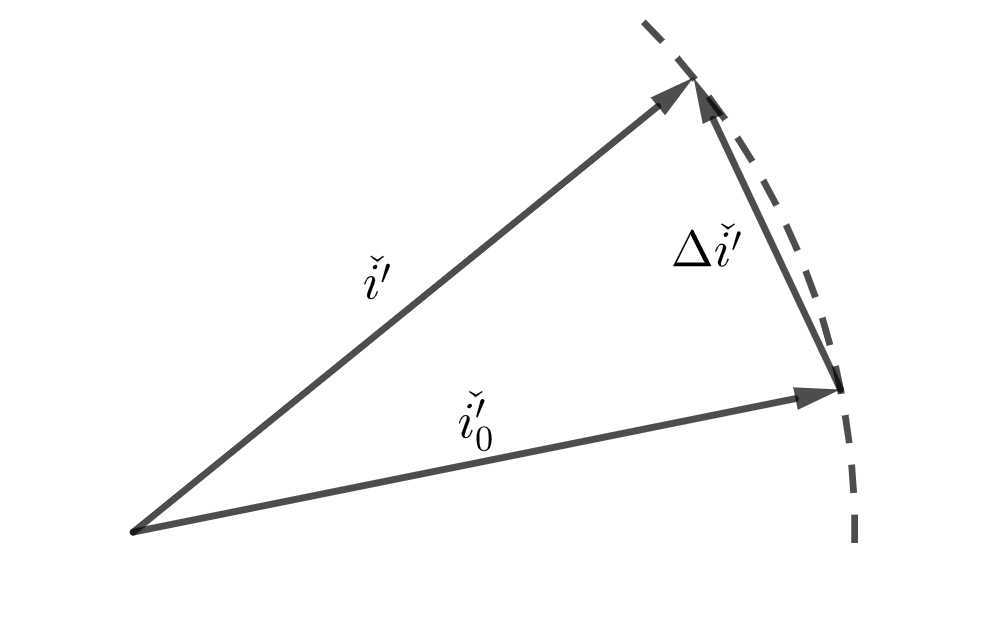
\includegraphics[scale=1.3]{../../common/img/62.01/theory/05-kinematics-rel-mov-rot-dv.png}
\label{fig:relMovRotDv}
\end{figure}

Observando la figura \ref{fig:relMovRotDv}, y considerando que la longitud de arco equivale al producto del ángulo por el radio, resulta, al tomar el límite:

\begin{equation}
\mathop{ d\check{i'} } = \mathop{ d\alpha } \underbrace{ ||\check{i'}|| }_{1} \check{j'}
\end{equation}

El hecho de que el diferencial de $\check{i'}$ tiene, como vector, la dirección $\check{j'}$ se observa geométricamente. Si se toma el límite, al acercarse $\check{i_0'}$ a $\check{i'}$, se observa que su dirección es ortogonal a la de $\check{i'}$. Como siguiente paso, en un abuso de notación, "dividiendo" miembro a miembro por $\mathop{dt}$, se tiene:

\begin{equation}
\frac{ \mathop{d \check{i'} } }{ \mathop{dt} } = \underbrace{ \frac{ \mathop{d\alpha} }{\mathop{dt}} }_{\omega} \check{j'}
\end{equation}

\begin{equation}
\tcboxmath[colback=orange!25!white,colframe=orange]{
\frac{ \mathop{d \check{i'} } }{ \mathop{dt} } = \omega \check{j'}
}
\end{equation}

Aplicando el mismo razonamiento para el versor $\check{j'}$, resulta entonces:

\begin{equation}
\tcboxmath[colback=orange!25!white,colframe=orange]{
\frac{ \mathop{d \check{j'} } }{ \mathop{dt} } = -\omega \check{i'}
}
\end{equation}

Es importante tener en cuenta que todo esto asume que el sentido de rotación de $S'$ es antihorario. Si el sentido fuera horario, las últimas dos igualdades tendrían el signo opuesto en $\omega$. Volviendo a la expresión de $\overrightarrow{r'}$:

\begin{subequations}
\begin{align}
\frac{ \mathop{ \overrightarrow{dr'} } }{ \mathop{dt} } &= \underbrace{ \frac{dx'}{dt} }_{v'_x} \check{i'} + x' \underbrace{ \frac{d\check{i'}}{dt} }_{\omega \check{j'}} + \underbrace{ \frac{dy'}{dt} }_{v'_y} \check{j'} + y' \underbrace{ \frac{d\check{j'}}{dt} }_{-\omega \check{i'}} \\
\frac{ \mathop{ \overrightarrow{dr'} } }{ \mathop{dt} } &= v'_x \check{i'} + x' \omega \check{j'} + v'_y \check{j'} + y' -\omega \check{i'}
\end{align}
\end{subequations}

Para el próximo paso, considérese el siguiente producto vectorial:

\begin{equation}
\overrightarrow{\omega} \times \overrightarrow{r'} = \det \begin{pmatrix}
\check{i'} & \check{j'} & \check{k'} \\
0 & 0 & \omega \\
x' & y' & 0
\end{pmatrix} = -y' \omega \check{i'} + x' \omega \check{j'}
\end{equation}

Reemplazando:

\begin{equation}
\frac{d\overrightarrow{r'}}{dt} = \underbrace{ v'_x \check{i'} + v'_y \check{j'} }_{\overrightarrow{v_{rel}}} + \underbrace{ \overrightarrow{\omega} \times \overrightarrow{r'} }_{?}
\end{equation}

¿Qué representa el segundo término? Puede pensarse como la velocidad de rotación del sistema móvil $S'$ respecto al sistema fijo $S$. Por ende, es la velocidad de arrastre.

Dado que $S'$ tiene siempre el mismo origen que $S$, en lo que concierne a $S$, $\overrightarrow{r} = \overrightarrow{r'}$ en todo instante. Por lo tanto, $\frac{d\overrightarrow{r}}{dt} = \frac{d\overrightarrow{r'}}{dt} = \overrightarrow{v_{abs}}$. Con lo que resulta finalmente:

\begin{equation}
\tcboxmath[colback=orange!25!white,colframe=orange]{
\vec{v}_{abs} = \underbrace{ v'_x \check{i'} + v'_y \check{j'} }_{\vec{v}_{rel}} + \underbrace{ \vec{\omega} \times \overrightarrow{r'} }_{\vec{v}_{arr}}
}
\end{equation}

Para obtener la aceleración, se deriva la velocidad. La derivada de $\vec{v}_{rel}$ es $\vec{a}_{rel}$, eso es trivial. Ahora bien, al derivar el producto vectorial del segundo término, se lo vuelve a expresar en términos de sus componentes, y se aplica la regla del producto:

\begin{equation}
\vec{a}_{abs} = \underbrace{ a'_x \check{i'} + a'_y \check{j'} }_{\vec{a}_{rel}} + \underbrace{ v'_x \omega \check{j'} - \omega v'_y \check{i'} }_{\vec{\omega} \times \vec{v'}} + \vec{\gamma} \times \vec{r} + \vec{\omega} \times \vec{v'}
\end{equation}

Finalmente, y sin perder de vista que este es el caso de sólo rotación:

\begin{equation}
\tcboxmath[colback=orange!25!white,colframe=orange]{
\vec{a}_{abs} = \vec{a}_{rel} + \underbrace{2 \vec{\omega} \times \vec{v'} }_{\text{ac. de Coriolis}} + \underbrace{ \vec{\gamma} \times \vec{r} }_{\vec{a}_{arr}}
}
\end{equation}

\section{Dinámica}

\subsection{Generalidades; 2da y 3ra leyes de Newton}

La dinámica es la rama de la física que estudia las causas del movimiento. Inicialmente, el modelo a seguir seguirá siendo el de partícula. Las causas serán interacciones (acciones mutuas) entre cuerpos, que pueden clasificarse de la siguiente manera:

\begin{itemize}
\item Fuertes: a nivel molecular. Pueden ser dentro del núcleo, o fuera del núcleo.
\item Débiles: producidas por campos. Esto incluye gravedad y electromagnetismo (por contacto o vínculo).
\end{itemize}

Nuestro estudio de la dinámica se centrará en las interacciones o fuerzas débiles.

\begin{itemize}
\item \textbf{Ley de las interacciones (3ra ley de Newton):} La característica principal de una interacción es la aparición de un par de fuerzas que actúan siempre en cuerpos distintos. Dichas fuerzas tienen igual dirección e intensidad, pero sentido opuesto.
\item \textbf{Vínculo}: Todo aquello que le quita libertad de movimiento a los cuerpos. Por ejemplo: mesa, piso, techo, soga, cadena, otro cuerpo.
\item \textbf{2da ley de Newton:} Para cada cuerpo, la suma vectorial de las fuerzas aplicadas sobre el mismo, o sea el vector fuerza resultante, equivale a la masa del cuerpo multiplicada por su vector aceleración. Matemáticamente:

\begin{equation}
\sum \vec{F} = \vec{F}_R = m \vec{a}
\end{equation}

En el contexto de la mecánica clásica, también llamada usualmente mecánica newtoniana, la masa se entiende como la cantidad de materia de un cuerpo, y es una magnitud escalar. En otros contexto como la mecánica cuántica, esa definición puede ser diferente. En esta materia, nos limitaremos a la definición newtoniana.

\item Pasos generales para resolver un problema de dinámica:

\begin{enumerate}
\item DCL: Diagrama de cuerpo libre. Indicar para cada cuerpo, las fuerzas que actúan como vectores.
\item Definir sistema de referencia, y sistema de coordenadas.
\item Para cada cuerpo, plantear la 2da ley de Newton, y resolver el sistema de ecuaciones resultante.
\end{enumerate}

\end{itemize}

\subsection{Rozamiento}

La fuerza de rozamiento aparece cuando una fuerza intenta cambiar el estado de movimiento de un cuerpo. Es una interacción: siempre habrá dos fuerzas iguales y opuestas en sentido. El vector $\vec{f}_r$ tiene, por convención, sentido opuesto al deslizamiento relativo entre las dos superficies.

El rozamiento puede ser \textbf{estático} o \textbf{dinámico}. El estático aplica cuando los cuerpos en contacto están sometidos a fuerzas no nulas, pero aún no hay movimiento relativo entre ambos. Para que empiece a haber movimiento, hay que vencer la fuerza de rozamiento estática. Por oposición, el rozamiento dinámico aparece cuando ya hay movimiento relativo entre los cuerpos. Como cabe esperar, los coeficientes de rozamiento son diferentes en ambos casos. Además, dependerán de los materiales de los cuerpos en contacto. Por ejemplo, hay coeficiente estático madera-madera, coeficiente estático madera-hierro, coeficiente dinámico madera-acero, etc.

\begin{figure}[ht]
\centering
\caption{Rozamiento}
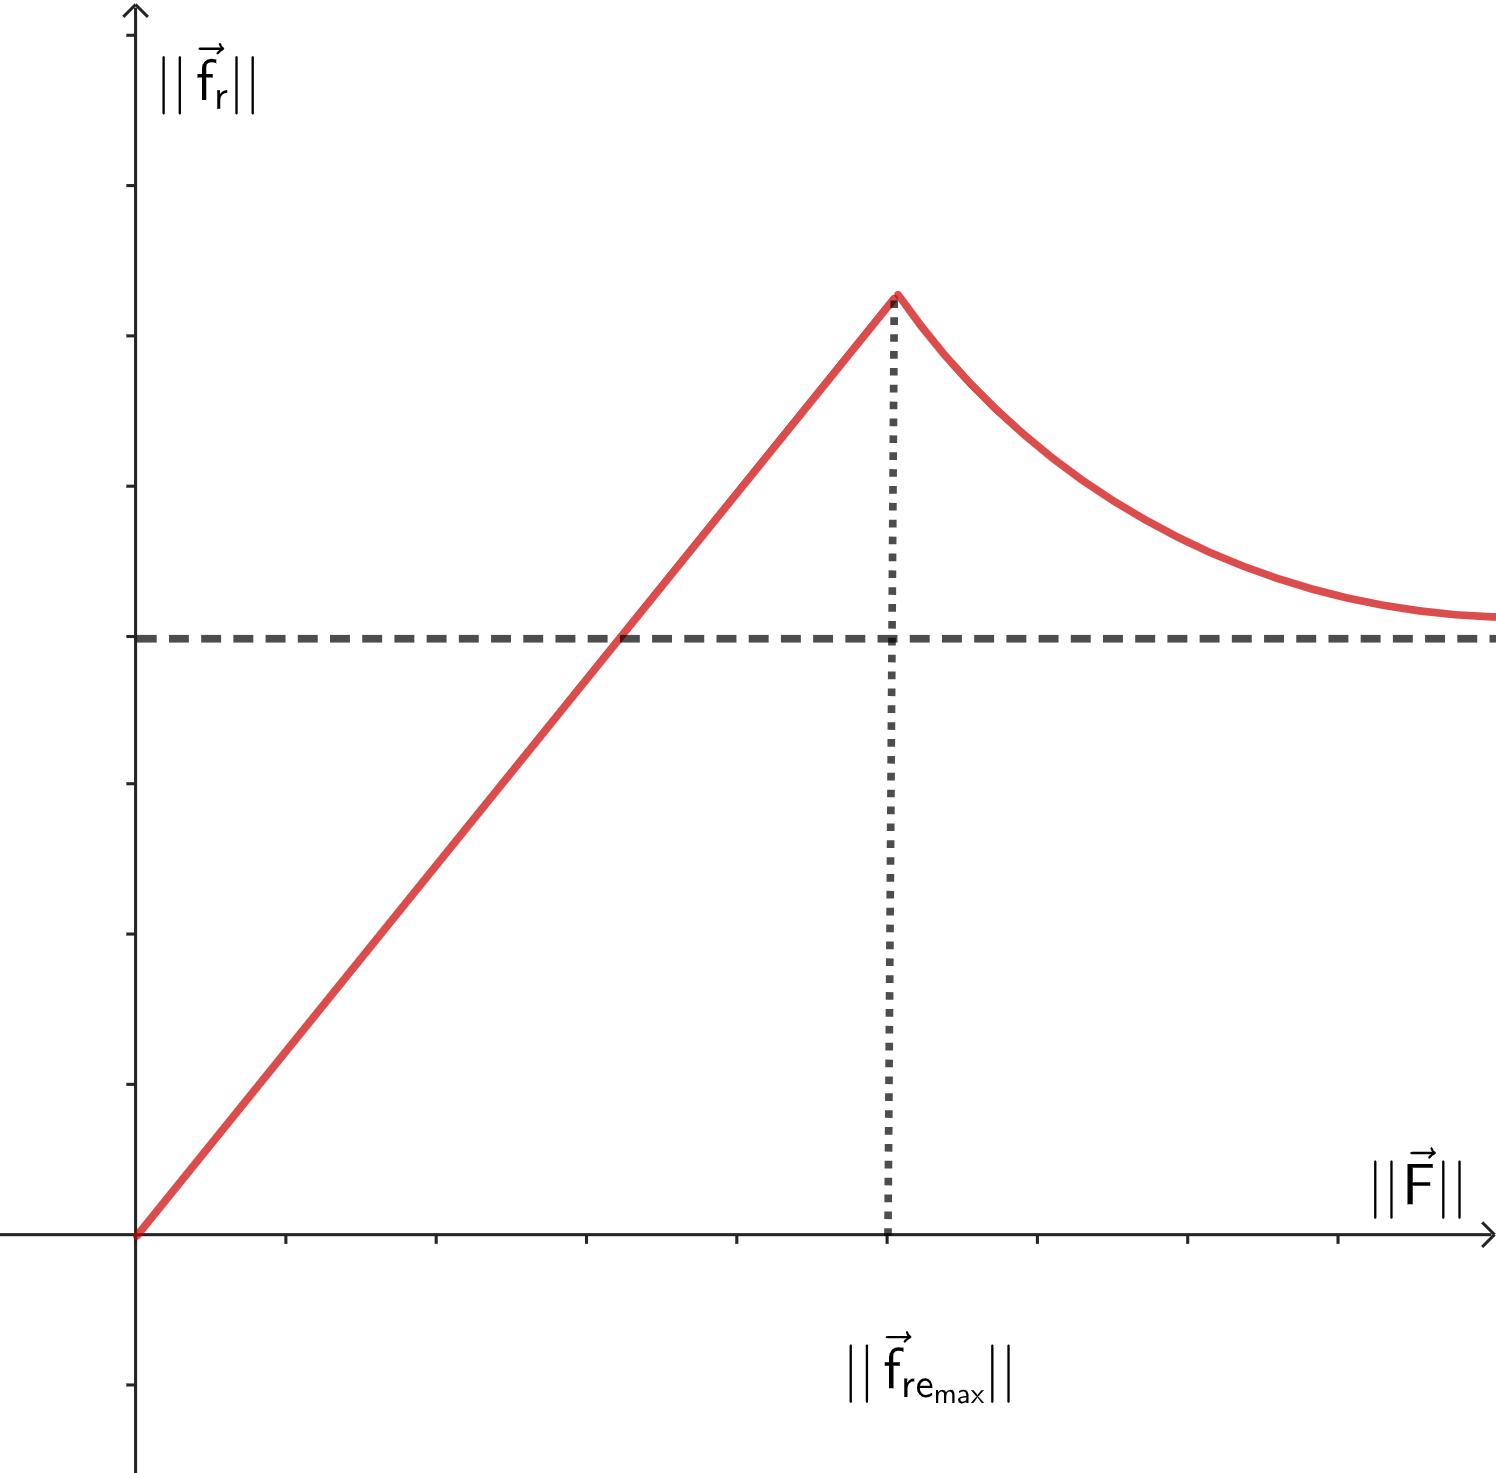
\includegraphics[scale=3.0]{../../common/img/62.01/theory/06-dynamics-friction.png}
\label{fig:friction}
\end{figure}

Si se grafica la intensidad de la fuerza aplicada al cuerpo contra la intensidad de la fuerza de rozamiento, suele seguir una curva como la de la figura \ref{fig:friction}. La intensidad de las fuerzas es lineal hasta que se llega a la intensidad máxima de rozamiento estático. Ese es el punto en que se pasa de rozamiento estático a dinámico. De ahí en adelante, la fuerza de rozamiento decae, pero tiende asintóticamente hacia una intensidad mínima. Vale decir, siempre habrá rozamiento.

De manera general, la intensidad de la fuerza de rozamiento está asociada a la intensidad de la normal y al coeficiente de rozamiento, según:

\begin{equation}
\tcboxmath[colback=orange!25!white,colframe=orange,title=Roz. estático]{
||\vec{f}_{re_{max}}|| = \mu_e ||\vec{N}||
}
\end{equation}

\begin{equation}
\tcboxmath[colback=orange!25!white,colframe=orange,title=Roz. dinámico]{
||\vec{f}_{rd}|| \approx \mu_d ||\vec{N}||
}
\end{equation}

En tanto se esté en rozamiento estático, $||\vec{f}_{re}|| \leq ||\vec{f}_{re_{max}}||$. El hecho de que una normal más intensa implica mayor fuerza de rozamiento estática máxima se condice con el hecho de que es más difícil poner en movimiento cuerpos de mayor masa. 

Si $||\vec{F}|| = ||\vec{f}_{re_{max}}||$, el cuerpo se mueve a velocidad constante. 

Por último, una forma intuitiva de calcular los coeficientes de rozamiento es pensar que $\mu \propto \frac{\text{ptos de contacto}}{\text{superficie}}$. Un par de superficies lisas tendrán un área de contacto casi igual a su superficie de contacto, y por ende tenderán a un coeficiente cercano a 1, que representa la ausencia de rozamiento. Por otro lado, un par de superficies más rugosas o disímiles entre sí tendrán menos puntos de contacto y por ende más fricción.

\subsection{Viscosidad}

Dado un cuerpo en movimiento dentro de un fluido, la viscosidad es una fuerza que se opone al movimiento del cuerpo. En particular, y en casos donde sea relevante, el aire puede ser considerado un fluido. Una forma básica de modelar la viscosidad es la siguiente:

\begin{equation}
\tcboxmath[colback=orange!25!white,colframe=orange,title=Viscosidad]{
\vec{F}_{rv} = -k \vec{v}
}
\end{equation}

El sufijo rv corresponde a un nombre alternativo de la fuerza viscosidad: resistencia viscosa. La constante $k$ depende del fluido, y $\vec{v}$ es, como cabe esperar, la velocidad del cuerpo. A continuación, se verá un ejemplo que combina rozamiento y viscosidad, y analiza el concepto de \textbf{velocidad crítica}.

Sea un cuerpo rectangular de masa $m$, modelado como partícula, sujeto a una fuerza externa conocida $\vec{F}$. Dicho cuerpo se encuentra apoyado sobre una superficie con rozamiento dinámico $\mu_{d}$, y dentro de un fluido con viscosidad $k$. Esta situación se grafica en la figura \ref{fig:viscosity}.

\begin{figure}[ht]
\centering
\caption{Viscosidad}
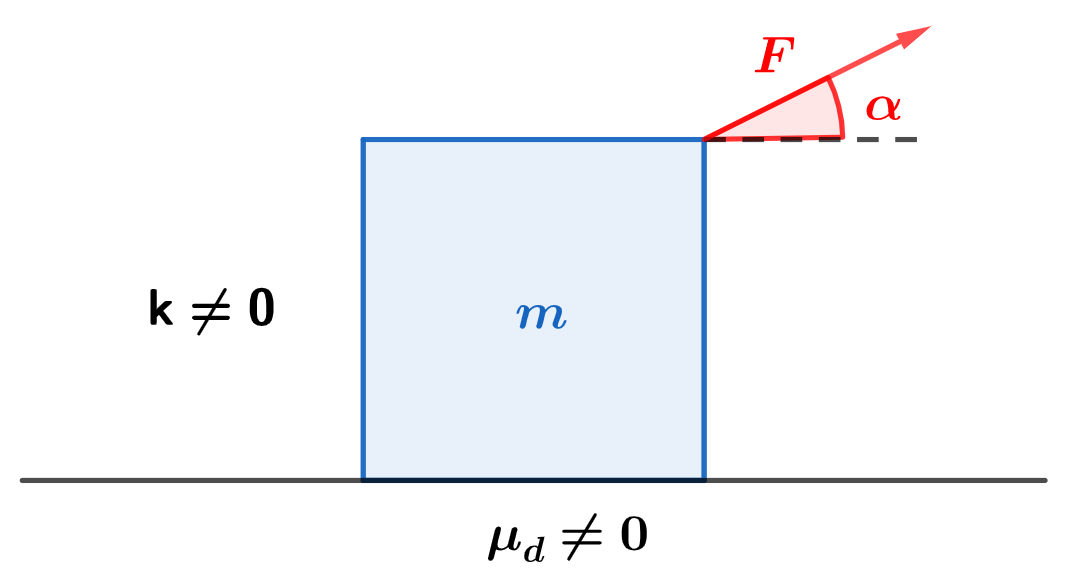
\includegraphics[scale=1.0]{../../common/img/62.01/theory/07-dynamics-viscosity-example.png}
\label{fig:viscosity}
\end{figure}

Modelando el cuerpo como partícula, se obtiene el diagrama de cuerpo libre de la figura \ref{fig:fbd}.

\begin{figure}[ht]
\centering
\caption{Viscosidad - DCL}
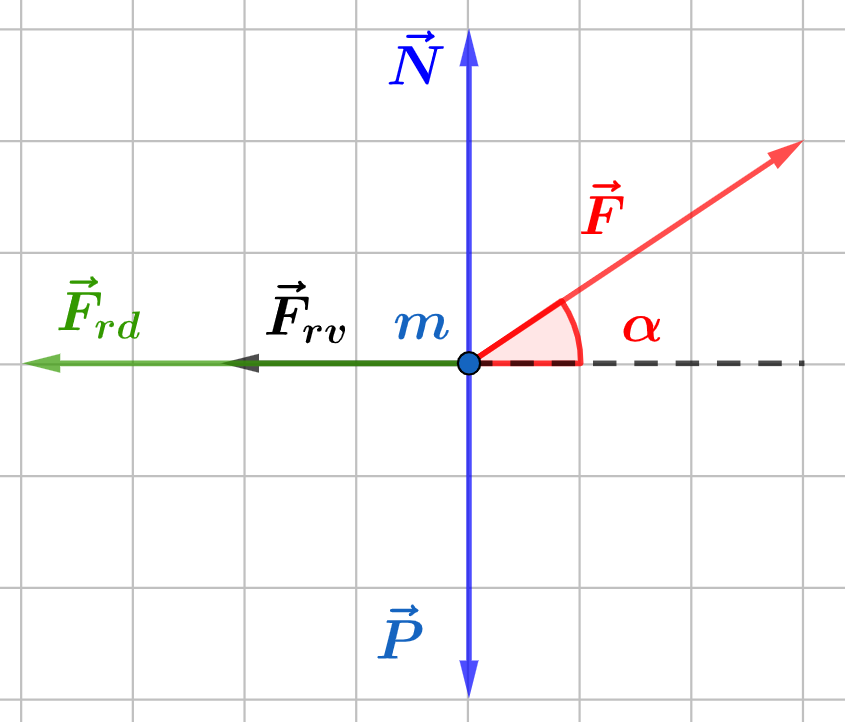
\includegraphics[scale=1.0]{../../common/img/62.01/theory/07-dynamics-viscosity-fbd.png}
\label{fig:fbd}
\end{figure}

Dado que el cuerpo está apoyado en un plano horizontal, y tiene una masa $m$, se plantean la fuerza peso $\vec{P}$, y la normal del plano horizontal $\vec{N}$. En color rojo se observa la fuerza externa $\vec{F}$. Dado que, para una partícula, dicha fuerza producirá un movimiento horizontal paralelo al plano, las fuerzas de rozamiento dinámico ($\vec{F}_{rd}$) y viscosidad ($\vec{F}_{rv}$) tienen vectores dirección opuestos a los del movimiento del objeto. Se dibujó $\vec{F}_{rd}$ como si tuviera mayor módulo que $\vec{F}_{rd}$ de manera arbitraria e ilustrativa; puede darse el caso opuesto, y ello se sabrá al resolver el sistema.

El segundo paso es definir un sistema de referencia. El mismo se define como un par de ejes cartesianos $x$ e $y$ con origen en la posición inicial del cuerpo.

El tercer y último paso es plantear la segunda ley de Newton para las dos dimensiones del problema. En este punto, se asume que la fuerza $F$ es tal que sólo produce movimiento horizontal en el cuerpo. Vale decir, la aceleración en la componente $y$ es nula. Teniendo esto en cuenta, resulta:

\begin{subequations}
\begin{align}
\textbf{x)} & \quad F \cos(\alpha) - k v - \mu_d N = m a \\
\textbf{y)} & \quad N - P + F \sin(\alpha) = 0
\end{align}
\end{subequations}

Despejando $N$ en la ecuación $\textbf{y)}$:

\begin{equation}
N = P - F \sin(\alpha)
\end{equation}

Reemplazando en la ecuación $\textbf{x)}$:

\begin{equation}
F \cos(\alpha) - k v - \mu_d (P - F \sin(\alpha)) = m a
\end{equation}

Si la fuerza $\vec{F}$ es constante en el tiempo, su módulo $F$ y el ángulo $\alpha$ también lo son. Restringiendo la solución a ese caso y recordando que $P$ es conocida por ser el producto de la masa $m$ por la constante $g$, la única incógnita que queda es la aceleración del cuerpo en función del tiempo, y su velocidad. Expresando la aceleración como la derivada de la velocidad respecto al tiempo, se obtiene la siguiente ecuación diferencial:

\begin{equation}
F [\cos(\alpha) + \mu_d \sin(\alpha)] - \mu_d P - k v = m \frac{\mathop{dv}}{\mathop{dt}}
\end{equation}

En esta ecuación, la incógnita es la función $v(t)$. Nótese que dicha ecuación es de variables separables, dado que es posible poner $t$ y $dt$ de un lado de la igualdad, y $v$ y $dv$ del otro.

\begin{equation}
\mathop{dt} = \frac{m}{-k v + F [\cos(\alpha) + \mu_d \sin(\alpha) - \mu_d P]}
\end{equation}

Integrando de ambos lados y haciendo el cambio de variable $u = $ todo el denominador, se llega a que:

\begin{equation}
v = C e^{-\frac{k}{m} t} + F [\cos(\alpha) + \mu_d \sin(\alpha) - \mu_d P]
\end{equation}

En esta expresión final de la velocidad, la constante $C$ es de integración y se calcula usando las condiciones iniciales del problema. Nótese que la solución tiene un término transitorio exponencial que depende sólo de la viscosidad y de la masa, y un término permanente constante que depende de la fuerza aplicada, el rozamiento dinámico, la masa del objeto y la aceleración de la gravedad. Este término permanente es lo que se conoce como \textbf{velocidad crítica}: a partir de cierto instante de tiempo, el término exponencial pasa a ser despreciable, y a fines prácticos, la velocidad del cuerpo se mantiene constante. Este valor de tiempo se conoce como \textbf{tiempo crítico}, y suele tomarse como $\frac{5k}{m}$. Esto surge de la regla práctica de que dada la exponencial decreciente $e^{\tau t}$, pasadas $5 \tau$ unidades de tiempo, la exponencial es, a fines prácticos, cero. Por último, nótese que como cabe esperar, el tiempo crítico depende de la viscosidad y la masa del cuerpo.

\subsection{Vínculos}

En el contexto de la mecánica clásica o newtoniana, los \textbf{vínculos} o \textbf{restricciones} describen condiciones que limitan o determinan el movimiento de los objetos o sistemas en estudio. Pueden observarse varios ejemplos de vínculos en la figura \ref{fig:constraints}. En dicha figura, los vectores de color rojo representan posibles fuerzas externas, y las flechas curvadas verdes en el caso de la rótula indican las dos posibles direcciones de movimiento de la misma. Por otro lado, en el caso del empotramiento, el cuerpo empotrado está totalmente fijo. Naturalmente, esto no contempla casos donde la fuerza sobre el cuerpo sea tan grande que lo doble o quiebre; no se modelarán ese tipo de casos en esta materia, y se asumirá que el cuerpo empotrado soportará las fuerzas a las que sea sometido.

\begin{figure}[ht]
\centering
\caption{Vínculos}
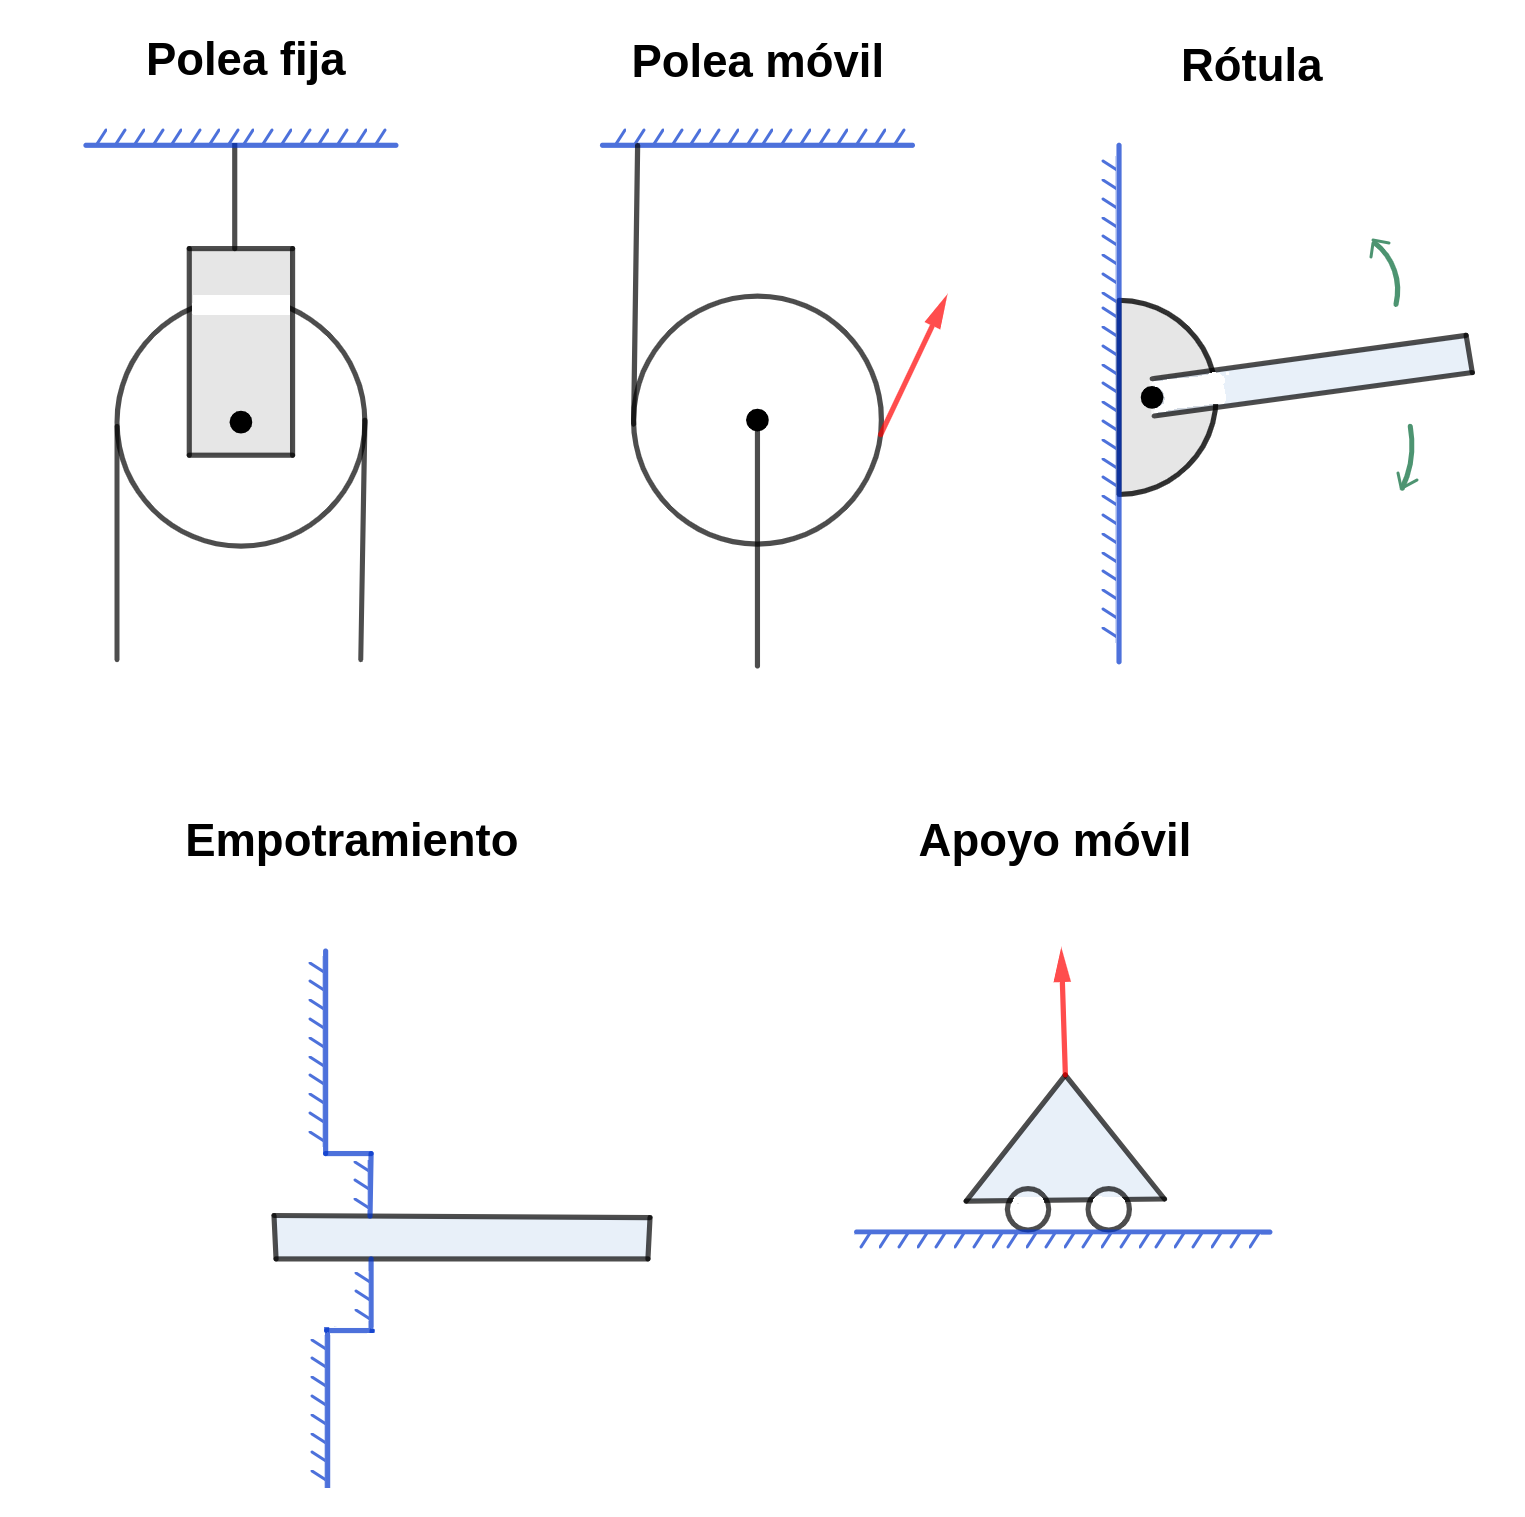
\includegraphics[scale=0.7]{../../common/img/62.01/theory/08-dynamics-constraints.png}
\label{fig:constraints}
\end{figure}

Otra consideración que se adoptará al lidiar con vínculos será la siguiente: las poleas, cadenas, cuerdas y demás cuerpos vinculados serán considerados inextensibles y de masa despreciable cuando su masa sea 10 veces menor que la de los demás cuerpos considerados. Este es un buen criterio general para sistemas mecánicos básicos.

\subsection{1ra ley de Newton: inercia}

Si la suma de fuerzas sobre un cuerpo es cero al menos en una dirección, en dicha dirección, si el cuerpo estaba en reposo permanecerá en reposo, y si se estaba moviendo continuará haciéndolo a velocidad constante. Recuérdese que para la suma de fuerzas también se utiliza el término \textbf{resultante}.

Si un sistema se mueve a velocidad constante, es equivalente a un \textbf{sistema inercial (SI)}. En cambio, si el sistema tiene una aceleración no nula, pasa a ser un \textbf{sistema no inercial (SNI)}.

Considérese el sistema de la figura \ref{fig:inertia}. Hay una barra de hielo apoyada sobre un camión. El camión tiene una aceleración no nula, y el rozamiento entre el hielo y el piso de la caja del camión es nulo.

\begin{figure}[ht]
\centering
\caption{Inercia - ejemplo}
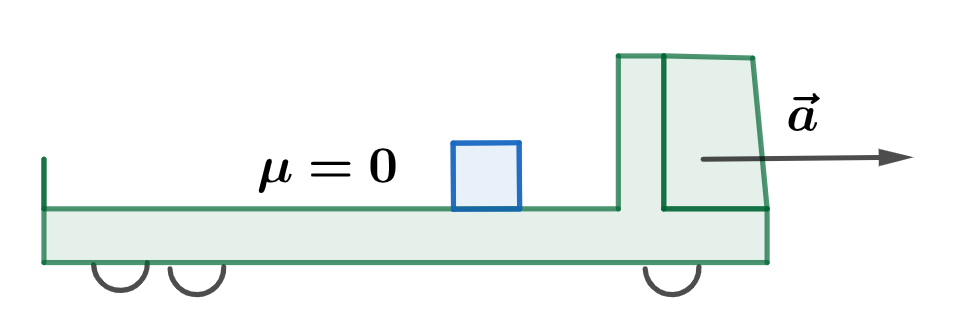
\includegraphics[scale=1.0]{../../common/img/62.01/theory/09-dynamics-inertia.png}
\label{fig:inertia}
\end{figure}

Si se observa sólo la barra de hielo tomando como referencia la tierra, la misma no se mueve: el camión avanzará y la barra resbalará hasta vincularse con el tope trasero de la caja del camión. Esto ocurre porque la tierra es un sistema inercial: para los fines de este problema, la tierra está en reposo y se cumple la 1ra ley, al menos hasta que la barra hace tope. Si se hiciera un diagrama de cuerpo libre de la barra de hielo en este caso, las únicas fuerzas serían el peso y la normal en la dirección y, y sumarían cero. En la dirección x no hay movimiento, al menos en el intervalo de interés (pre vínculo con tope trasero del camión).

Ahora bien, si se toma como sistema de referencia el camión, las fuerzas son las mismas, pero se observa un movimiento en la barra. Esto ocurre porque el sistema de referencia mismo está acelerado: es un \textbf{sistema de referencia no inercial (SRNI)}. Para que sigan valiendo las leyes de Newton, es preciso aplicar una fuerza ficticia a todo cuerpo del sistema. Dicha fuerza tendrá dirección opuesta a la aceleración del sistema, y su módulo será el producto de la masa del cuerpo en cuestión por el módulo de la aceleración del sistema. Para el caso de la barra, tomando como sistema de referencia el camión, el diagrama de cuerpo libre sería ahora el de la figura \ref{fig:inertia-example}.

\begin{figure}[ht]
\centering
\caption{Inercia - ejemplo - DCL}
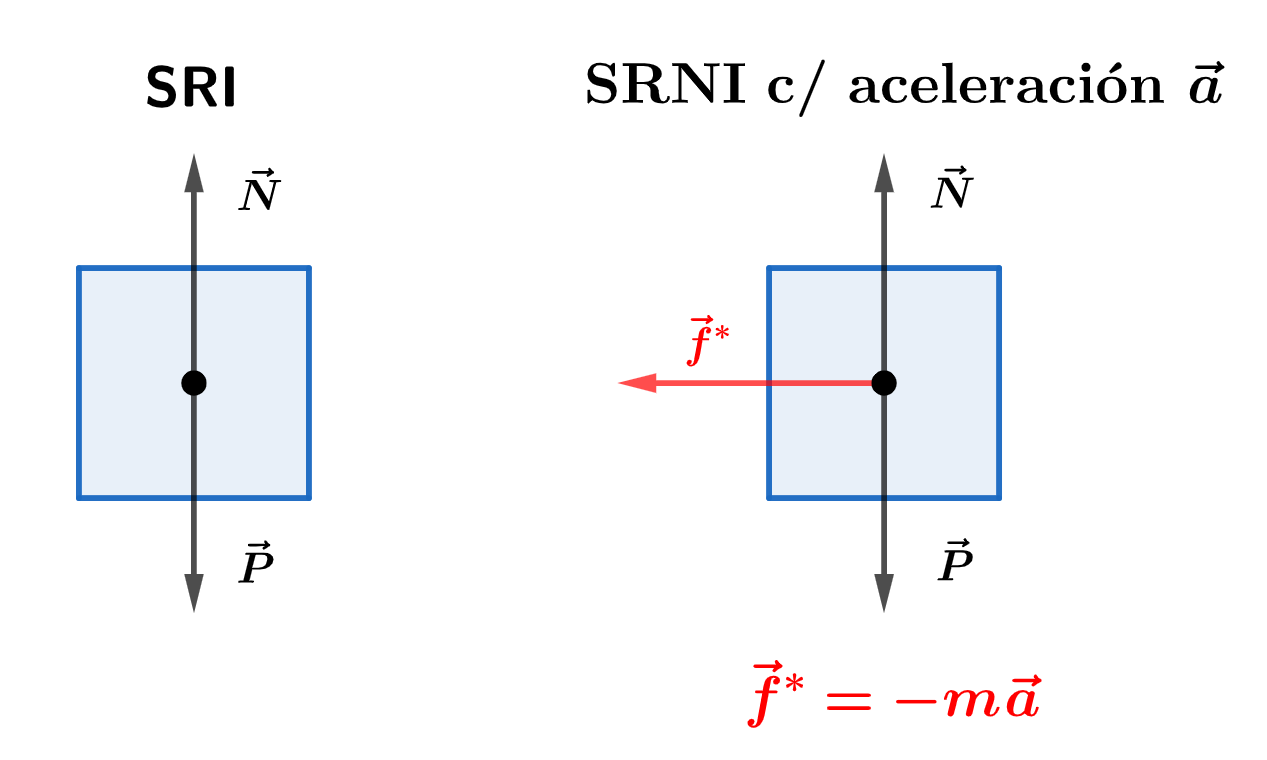
\includegraphics[scale=0.8]{../../common/img/62.01/theory/10-dynamics-inertia-example.png}
\label{fig:inertia-example}
\end{figure}

La fuerza ficticia $\vec{f}^{*}$ es la que justifica el movimiento observado en la barra de hielo cuando el sistema de referencia es el camión. Recuérdese que si hubiera más cuerpos, todos tendrían aplicada una fuerza ficticia proporcional a su masa.

\subsubsection{Péndulo cónico}

Éste es otro ejemplo de cómo un sistema puede verse como inercial o no inercial según el sistema de referencia adoptado. Observando el diagrama de la figura \ref{fig:conic-pendulum}, y asumiendo que no hay rozamiento u otros efectos que detengan el movimiento del péndulo, el cuerpo colgado de la cuerda realizará un movimiento circular en un plano horizontal. Esto requiere que la cuerda sea larga, flexible, sin masa e inextensible (que no se estire).

Si en primer lugar se toma como referencia la tierra, se tiene un sistema inercial. Concretamente, se define el eje x dentro del plano de movimiento y el eje y, perpendicular. Nótese que con este esquema, sólo se observa la posición del cuerpo en la proyección lateral del plano, no en las dos coordenadas que tendría si se observara el movimiento que realiza desde arriba. Con este sistema de referencia, fijo e inercial, y en las condiciones dadas, se observa movimiento y aceleración en la dirección x. En la dirección y, el peso del cuerpo es compensado por la componente y de la tensión en la cuerda.

\begin{figure}[ht]
\centering
\caption{Péndulo cónico - SI}
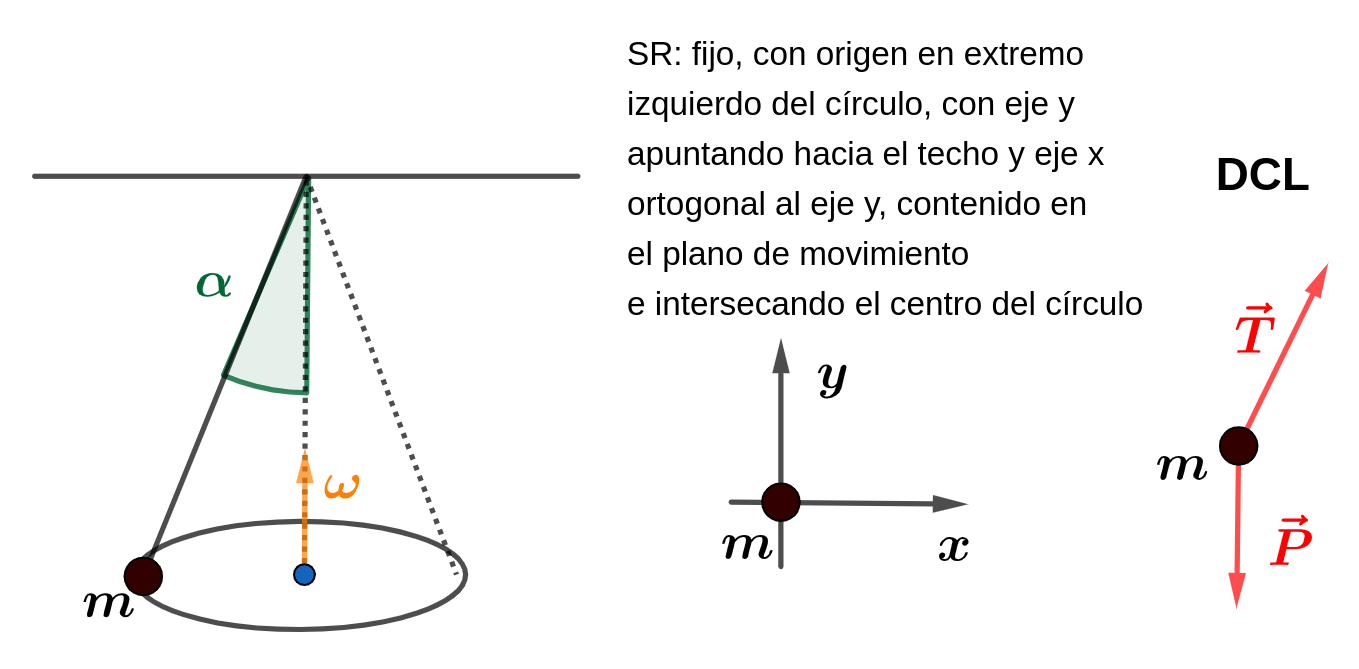
\includegraphics[scale=0.7]{../../common/img/62.01/theory/11-dynamics-conic-pendulum.png}
\label{fig:conic-pendulum}
\end{figure}

Por otro lado, dado que no hay pérdida de energía, el movimiento es infinito, por lo tanto $\alpha$ es constante y en consecuencia $\omega$ también. Con eso en mente, las ecuaciones de Newton resultan:

\begin{subequations}
\begin{align}
\textbf{x)} & \quad T \sin(\alpha) = m a_n \\
\textbf{y)} & \quad T \cos(\alpha) - P = 0
\end{align}
\end{subequations}

Ahora bien, si este mismo problema se plantea poniendo el sistema de referencia en el cuerpo suspendido del péndulo, el sistema pasa a ser no inercial. Cabe aclarar que en ese caso, el eje y seguiría apuntando al techo, en tanto el eje x pasaría a apuntar siempre hacia el centro del círculo. Por otro lado, el origen se movería siguiendo la posición del cuerpo. Teniendo en cuenta todo esto, el planteamiento pasa a ser el de la figura \ref{fig:conic-pendulum-ni}.

\begin{figure}[ht]
\centering
\caption{Péndulo cónico - SNI}
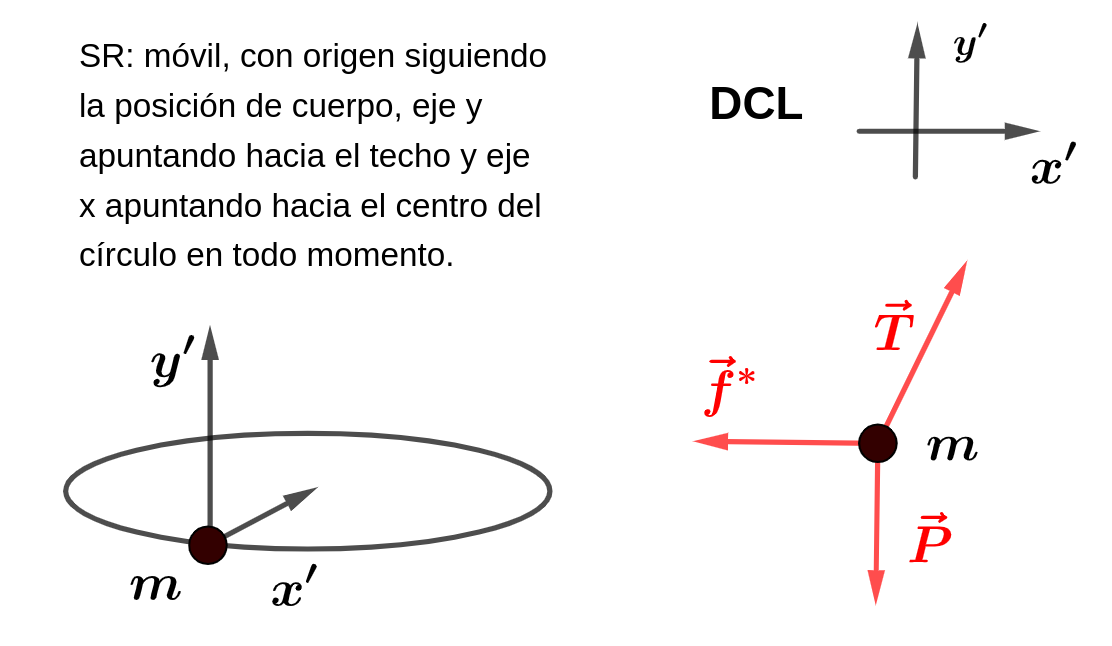
\includegraphics[scale=0.7]{../../common/img/62.01/theory/12-dynamics-conic-pendulum-ni.png}
\label{fig:conic-pendulum-ni}
\end{figure}

Nótese la aparición de la fuerza ficticia $\vec{f}^{*}$, en el sentido opuesto al de la aceleración centrífuga que experimenta el sistema de referencia. Dicha fuerza tendrá módulo igual a $m a_n$.

\subsubsection{Péndulo ideal}

Así como el péndulo cónico mueve el objeto suspendido en un plano horizontal, el péndulo ideal lo hace en un plano vertical, como se observa en la figura \ref{fig:ideal-pendulum}, en la cual, típicamente, se conocen el largo del hilo, $L$, y la masa del objeto, $m$. Para simplificar, el hilo se considera de masa despreciable comparada a la del objeto.

\begin{figure}[ht]
\centering
\caption{Péndulo ideal}
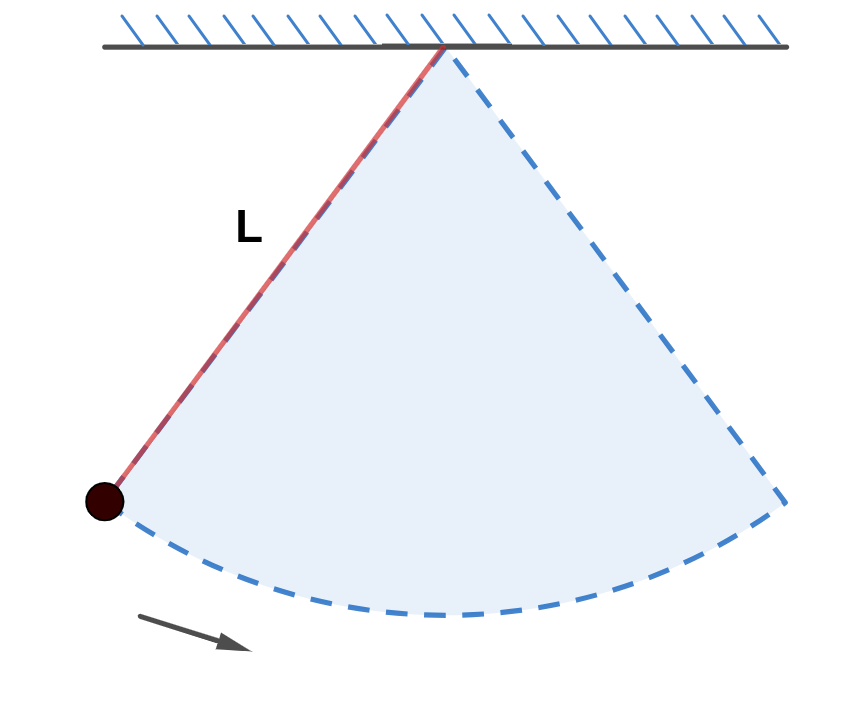
\includegraphics[scale=0.7]{../../common/img/62.01/theory/13-dynamics-ideal-pendulum.png}
\label{fig:ideal-pendulum}
\end{figure}

En un planteamiento no inercial, el sistema de referencia estaría en el objeto, con un sistema de coordenadas intrínseco: un eje en la direcciones normal y otro en la tangente, instante a instante. Esto conduciría a un diagrama de cuerpo libre como el de la figura \ref{fig:ideal-pendulum-ni}.

\begin{figure}[ht]
\centering
\caption{Péndulo ideal - SI}
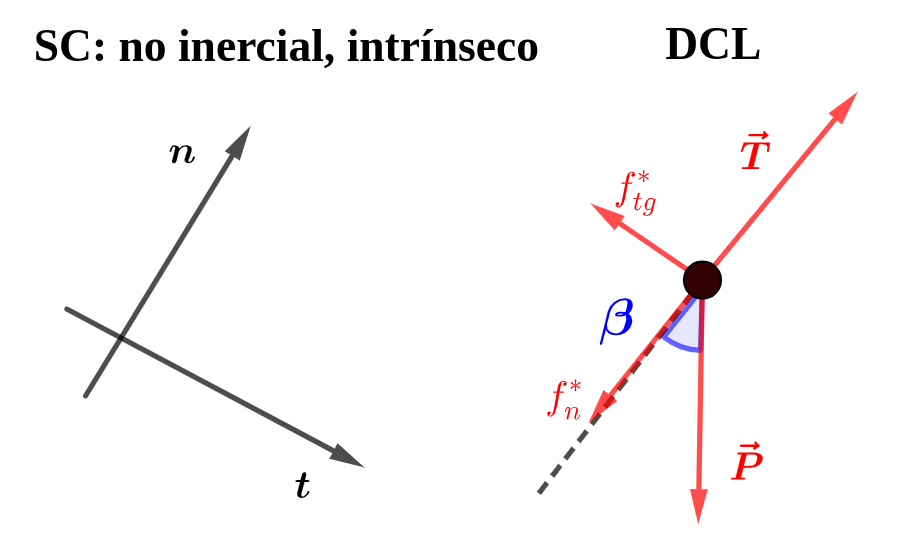
\includegraphics[scale=1]{../../common/img/62.01/theory/14-dynamics-ideal-pendulum-ni.png}
\label{fig:ideal-pendulum-ni}
\end{figure}

Con este sistema de referencia, el sistema de referencia presenta fuerzas ficticias en la dirección normal, y aceleración tangencial en la dirección homónima. Dichas fuerzas se oponen al sentido de la aceleración. Ello conduce a las siguientes ecuaciones de Newton:

\begin{subequations}
\begin{align}
\textbf{n)} & \quad T - P \cos(\beta) - m a_n = 0 \\
\textbf{t)} & \quad P \sin(\beta) - m a_{tg} = 0
\end{align}
\end{subequations}

Para resolver este sistema, lo más sencillo es tomar la ecuación tangencial y notar que el ángulo $\beta$ es congruente con el ángulo $\theta$ del péndulo, y por ende son iguales. Luego, $P = m g$. Y por último, $a_{tg}(t) = \frac{d^2s}{dt^2}$, donde $s$ es la posición del objeto medida a lo largo del arco de círculo (cero es la posición de equilibrio). Ello conduce a:

\begin{subequations}
\begin{align}
P \sin(\beta) - m a_{tg} = 0 \\
m g \sin(\theta) - m \frac{d^2s}{dt^2} = 0
\end{align}
\end{subequations}

Ahora bien, la posición en el arco está relacionado con $\theta$ y la longitud del hilo: $s = L \theta$. Derivando respecto al tiempo miembro a miembro dos veces, siendo $L$ una constante, resulta que $\frac{d^2s}{dt^2} = L \frac{d^2\theta}{dt^2}$. Reemplazando, se llega a una ecuación diferencial cuya incógnita es la función $\theta(t)$.

\begin{subequations}
\begin{align}
mg \sin(\theta) = m L \frac{d^2\theta}{dt^2} \\
\frac{d^2\theta}{dt^2} = \frac{g}{L} \sin(\theta)
\end{align}
\end{subequations}

Esta ecuación es bastante compleja para resolver de manera algebraica, dado que la función $\theta$ está compuesta con una función seno. Para simplificar, se puede plantear que para valores pequeños de $\theta$, $\sin(\theta) \approx \theta$. Ello conduce a una ecuación de 2do orden típica donde la solución general es una combinación lineal de un seno y coseno de cierta frecuencia.

\subsection{Resortes}

Para simplificar el modelado, los resortes se considerarán sin masa. Cada resorte está caracterizado por una constante $k$, que depende de la longitud, el número de espiras, el material y demás características físicas.

Otra consideración que se hará a la hora de resolver problemas es que las cargas o fuerzas aplicadas al resorte no lo quitarán de su período elástico. Cuando la fuerza aplicada sobre el resorte es demasiado grande, el mismo deja de comportarse linealmente. Además, puede que sufra modificaciones permanentes y su respuesta quede alterada. Un gráfico de este concepto puede apreciarse en la figura \ref{fig:spring-01}.

\begin{figure}[ht]
\centering
\caption{Resorte ideal}
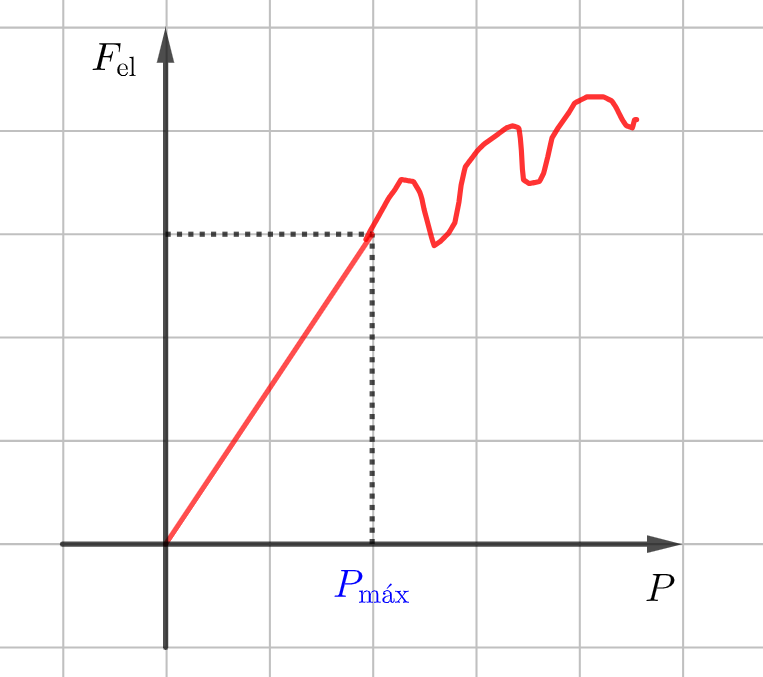
\includegraphics[scale=0.8]{../../common/img/62.01/theory/15-dynamics-spring-01.png}
\label{fig:spring-01}
\end{figure}

Supóngase el escenario relativamente trivial de un resorte colgando del techo, del cual se cuelga una masa $m$, como se ve en la figura \ref{fig:spring-02}. Para resolver cualquier problema de resortes donde se aplique el modelo simple establecido, se aplicará la ley de Hooke, verbigracia:

\begin{figure}[ht]
\centering
\caption{Resorte ideal - ejemplo}
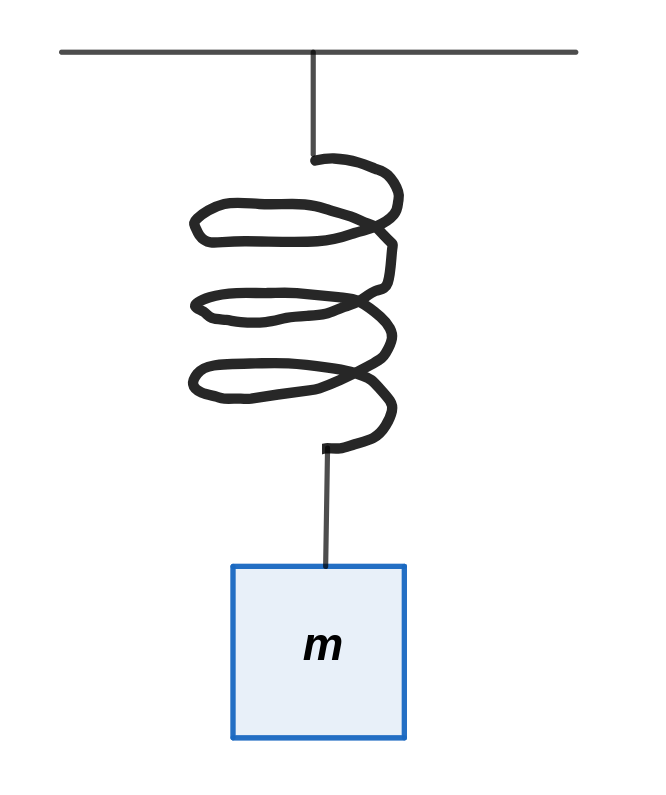
\includegraphics[scale=0.8]{../../common/img/62.01/theory/15-dynamics-spring-02.png}
\label{fig:spring-02}
\end{figure}

\begin{equation}
\tcboxmath[colback=orange!25!white,colframe=orange,title=Ley de Hooke]{
\quad \overrightarrow{F_{\text{el}}} = -k \mathop{\overrightarrow{\Delta x}} \quad
}
\end{equation}

Esta ley indica que la fuerza elástica generada sobre el resorte será proporcional al estiramiento que se le aplique, y en la dirección opuesta`. El estiramiento estará dado por la diferencia vectorial entre la posición inicial y la posición final: $\mathop{\overrightarrow{\Delta x}} = \overrightarrow{x_f} - \overrightarrow{x_i}$.

Volviendo al problema de ejemplo, sobre el cuerpo colgado del resorte operarán entonces la fuerza peso y la fuerza elástica; la segunda se aplica sobre el cuerpo por estar el mismo vinculado al resorte. Véase el diagrama de cuerpo libre de la figura \ref{fig:spring-03}.

\begin{figure}[ht]
\centering
\caption{Resorte ideal - ejemplo - DCL}
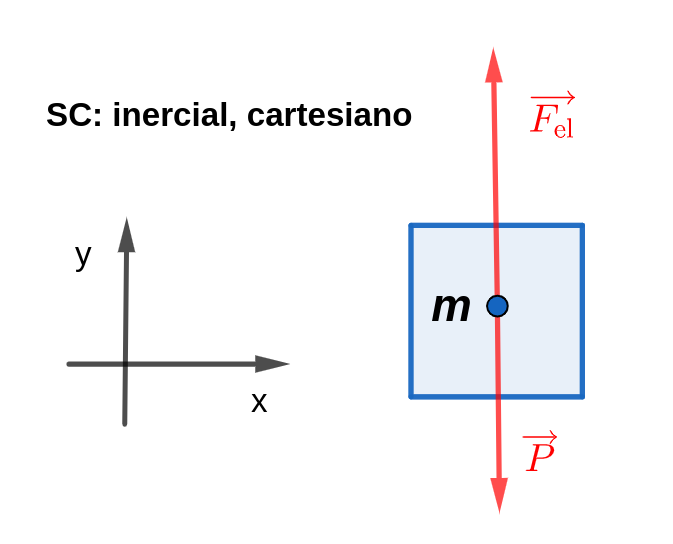
\includegraphics[scale=0.8]{../../common/img/62.01/theory/15-dynamics-spring-03.png}
\label{fig:spring-03}
\end{figure}

Este sistema estará gobernado por la ley de Hooke, instante a instante, en tanto el peso del cuerpo esté dentro del período elástico del resorte.

\subsection{Trabajo y energía}

\subsubsection{Trabajo}

Las ecuaciones de Newton son suficientes para un instante de tiempo específico, aceleración constante, o si se sabe previamente cómo varía la aceleración. Para los demás casos, ayuda pensar en términos de una nueva magnitud: el trabajo. Esta magnitud suele denotarse con la letra $W$, y puede definirse de varias maneras. Una muy útil es la siguiente:

\begin{equation}
\tcboxmath[colback=orange!25!white,colframe=orange,title=Trabajo]{
W = \oint_{r_0}^{r_f} \overrightarrow{F} \cdot \overrightarrow{\mathop{dr}} = \int_{x_0}^{x_f} F_x \mathop{dx} + \int_{y_0}^{y_f} F_y \mathop{dy} + \int_{z_0}^{z_f} F_zx \mathop{dz}
}
\end{equation}

Como caso particular, si $\overrightarrow{F}$ es constante en módulo y dirección:

\begin{equation}
\overrightarrow{F} = \text{cte} \Rightarrow W = \overrightarrow{F} \cdot \overrightarrow{\mathop{\Delta r}} = |F| |\mathop{\Delta r}| \cos( \alpha(\overrightarrow{F}, \overrightarrow{\mathop{\Delta r}}) )
\end{equation}

Nótese que la integral es curvilínea, y se aplica sobre el producto escalar entre la fuerza y el desplazamiento. Además, se descompuso en coordenadas cartesianas, pero bien podrían utilizarse coordenadas cilíndricas, esféricas, polares, según convenga.

Conceptualmente, el trabajo es una forma de energía. Más específicamente, el trabajo es realizado cuando una fuerza actúa sobre un cuerpo que se desplaza de una posición a otra. La fuerza puede variar punto a punto, vale decir ser una función de la posición del cuerpo. Se dice que el trabajo es realizado por una fuerza, en tanto la energía pertenece a un cuerpo.

En cuanto a unidades, siempre van a ser un producto entre unidades de fuerza y de distancia. Algunas posibilidades son:

\begin{itemize}
\item $[W] = N \cdot m = J$ (Newton-metro = Joule)
\item $[W] = \text{dyn} \cdot \text{cm} = \text{Erg}$ (Dina-centímetro = Ergio)
\item $[W] = \overrightarrow{\text{kg}} \cdot m$ (kilográmetros)
\end{itemize}

El trabajo $W$ puede ser:

\begin{itemize}
\item Positivo: en este caso, se denomina \textbf{trabajo motor}. Cuando el ángulo entre fuerza y desplazamiento es cero, se tiene el máximo trabajo motor posible.
\item Negativo: en este caso, se denomina \textbf{trabajo resistente}. Cuando el ángulo entre fuerza y desplazamiento es de 180 grados, se tiene el máximo trabajo resistente posible.
\item Nulo: esto ocurre cuando los vectores fuerza y desplazamiento son ortogonales.
\end{itemize}

\subsubsection{Energía cinética}

Dado un cuerpo de masa $m$ que se mueve con velocidad $\overrightarrow{v}$ en un instante de tiempo, su energía cinética está dada por:

\begin{equation}
\tcboxmath[colback=orange!25!white,colframe=orange,title=Energía cinética]{
\quad E_c = \frac{1}{2} m ||\overrightarrow{v}||^2 \quad
}
\end{equation}

\subsubsection{Teorema de las fuerzas vivas}

Este teorema establece que el trabajo de la fuerza resultante es igual a la variación de energía cinética. Por otro lado, el trabajo de la fuerza resultante es equivalente a la suma del trabajo realizado por cada fuerza. Algebraicamente:

\begin{equation}
\tcboxmath[colback=orange!25!white,colframe=orange,title=Teorema de las fuerzas vivas]{
\sum W = \Delta E_c \Leftrightarrow W_{F_{\text{res}}} = \Delta E_c
}
\end{equation}

\subsection{Fuerzas conservativas y no conservativas}

Se dice que una fuerza es conservativa si y sólo si el trabajo que realiza en toda trayectoria cerrada es cero. Estas fuerzas surgen de campos conservativos. En este curso, sólo la fuerza peso y la fuerza elástica serán consideradas conservativas. De manera más abarcativa, cualquier otro tipo de fuerza será considerada no conservativa hasta que se demuestre lo contrario.

Que una fuerza sea conservativa tiene dos fuertes consecuencias:

\begin{enumerate}
\item Dados dos puntos A y B, el trabajo realizado por una fuerza conservativa en el trayecto de ida es igual y opuesto al trabajo del trayecto de vuelta. Simbólicamente, $W_{AB} = -W_{BA}$.

\item Dados dos puntos A y B, el trabajo realizado por una fuerza conservativa no depende de la trayectoria elegida. Por lo tanto, en tanto una A con B, se puede elegir el camino que más facilite los cálculos.
\end{enumerate}

Se dice que un sistema físico es conservativo cuando no hay fuerzas no conservativas que realicen trabajo.

\subsubsection{Energía potencial}

Asociada a toda fuerza conservativa, hay energía potencial. Para la fuerza peso, se tiene la energía potencial gravitatoria, $E_{\text{pg}}$. Para un cuerpo de masa $m$ ubicado a una altura $h$:

\begin{equation}
\tcboxmath[colback=orange!25!white,colframe=orange,title=Energía potencial gravitatoria]{
\quad \quad \quad \quad E_{\text{pg}} = m g h + c \quad \quad \quad \quad
}
\end{equation}

La constante $c$ se refiere a la posición del cero potencial. Esto se elige arbitrariamente como referencia, suele ser el nivel del suelo y suele asignarse $c = 0$. En todo caso, la posición y valor del cero potencial gravitatoria siempre debe explicitarse al resolver un problema que involucre esta magnitud.

Adicionalmente, para alturas pequeñas, puede demostrarse que:

\begin{equation}
\tcboxmath[colback=orange!25!white,colframe=orange]{
\Delta E_p = -W_{FC}
}
\end{equation}

Para el caso de un resorte con constante $k$ al que se ha aplicado un estiramiento $\mathop{\Delta x}$, la energía potencial elástica está dada por:

\begin{equation}
\tcboxmath[colback=orange!25!white,colframe=orange,title=Energía potencial elástica]{
\quad \quad \quad E_{\text{pel}} = \frac{1}{2} k \mathop{\Delta x}^2 \quad \quad \quad
}
\end{equation}

\subsubsection{Conservación de energía mecánica}

Partiendo del teorema de las fuerzas vivas, vale decir:

\begin{equation}
\sum W = \Delta E_c
\end{equation}

En el lado izquierdo de la igualdad, la suma del trabajo puede descomponerse en el trabajo realizado por fuerzas conservativas, y el trabajo realizado por fuerzas no conservativas.

\begin{equation}
\sum W_{FC} + \sum W_{F\cancel{C}} = \Delta E_c
\end{equation}

Asumiendo que las alturas involucradas son pequeñas, vale la igualdad $\Delta E_p = -W_{FC}$. Reemplazando:

\begin{equation}
-\Delta E_p + \sum W_{F\cancel{C}} = \Delta E_c
\end{equation}

Pasando la energía potencial al lado derecho:

\begin{equation}
\sum W_{F\cancel{C}} = \underbrace{ \Delta E_c + \Delta E_p }_{\Delta E_m}
\end{equation}

A la suma de energía potencial y energía cinética se la denomina \textbf{energía mecánica}, y esta denominación se extiende naturalmente a su variación o $\Delta$. Finalmente, recordando que las alturas consideradas deben ser pequeñas, se tiene el resultado:

\begin{equation}
\tcboxmath[colback=orange!25!white,colframe=orange,title=Energía mecánica]{
\quad \sum W_{F\cancel{C}} = \Delta E_m \quad
}
\end{equation}

Como caso particular, considérese $\Delta E_m = 0$. Esto implica que la energía mećanica es constante, y por la igualdad anterior, la suma del trabajo de las fuerzas no conservativas es cero. Esto puede ocurrir por tres razones:

\begin{enumerate}
\item No hay fuerzas no conservativas, o se anulan entre sí.
\item No hay desplazamiento.
\item Las fuerzas no conservativas son ortogonales al desplazamiento.
\end{enumerate}

Volviendo a la expresión inicial del teorema de las fuerzas vivas, considerése el caso particular en que la energía cinética se conserva. Esto implicaría que $\sum W = 0$. De manera análoga, esto puede ocurrir por tres razones:

\begin{enumerate}
\item No hay fuerzas, o se anulan entre sí.
\item No hay desplazamiento.
\item Las fuerzas son ortogonales al desplazamiento.
\end{enumerate}

\subsection{Potencia}

La potencia es la rapidez con que se realiza el trabajo. Por lo tanto, se define como su derivada respecto al tiempo.

\begin{equation}
\tcboxmath[colback=orange!25!white,colframe=orange,title=Potencia]{
P = \frac{\mathop{dW}}{\mathop{dt}}
}
\end{equation}

Esta definición corresponde a la denominada \textbf{potencia instantánea}. También se puede hablar de \textbf{potencia media}, considerando un instante inicial y un instante final.

\begin{equation}
\tcboxmath[colback=orange!25!white,colframe=orange,title=Potencia media]{
\overline{P} = \frac{\mathop{\Delta W}}{\mathop{\Delta t}} = \frac{W_f - W_0}{t_f - t_0}
}
\end{equation}

Las unidades de potencia serán de energía sobre tiempo. Particularmente, $[P] = \frac{J}{s} = W$ (Watt). Cuando se habla de caballos de fuerza, se utiliza la equivalencia:

\begin{equation}
1 HP = 746 W
\end{equation}

\subsection{Rendimiento}

El rendimiento de un sistema físico es el cociente entre la energía que otorga, y la energía que se le brinda. Suele denotarse con la letra griega eta.

\begin{equation}
\eta = \frac{\text{Energia obtenida}}{\text{Energia entregada}}
\end{equation}

Naturalmente, este valor es adimensional y siempre será menor a 1, ya que nunca se obtendrá más energía de la entregada, y siempre habrá pérdidas por calor, fricción, etcétera. También suele ser especificado como porcentaje, en cuyo caso es simplemente el mismo valor multiplicado por 100.

\subsection{Momento de una fuerza}

El momento de una fuerza aplicada en un punto $\overrightarrow{P}$ respecto a un punto $\overrightarrow{O}$ se define como:

\begin{equation}
\tcboxmath[colback=orange!25!white,colframe=orange,title=Momento de una fuerza respecto a un punto]{
\overrightarrow{M_{F}^{O}} = (\overrightarrow{P}-\overrightarrow{O}) \times \overrightarrow{F} = \overrightarrow{r} \times \overrightarrow{F}
}
\end{equation}

Por ejemplo, si se está apretando un tornillo con una llave inglesa, el punto $\overrightarrow{O}$ sería la posición del tornillo, y el punto $\overrightarrow{P}$ sería el extremo de la llave en el cual se la toma con la mano y se aplica la fuerza $\overrightarrow{F}$. Un ejemplo en 3 dimensiones se vería como la figura \ref{fig:torque-01}.

\begin{figure}[ht]
\centering
\caption{Momento de una fuerza respecto a un punto}
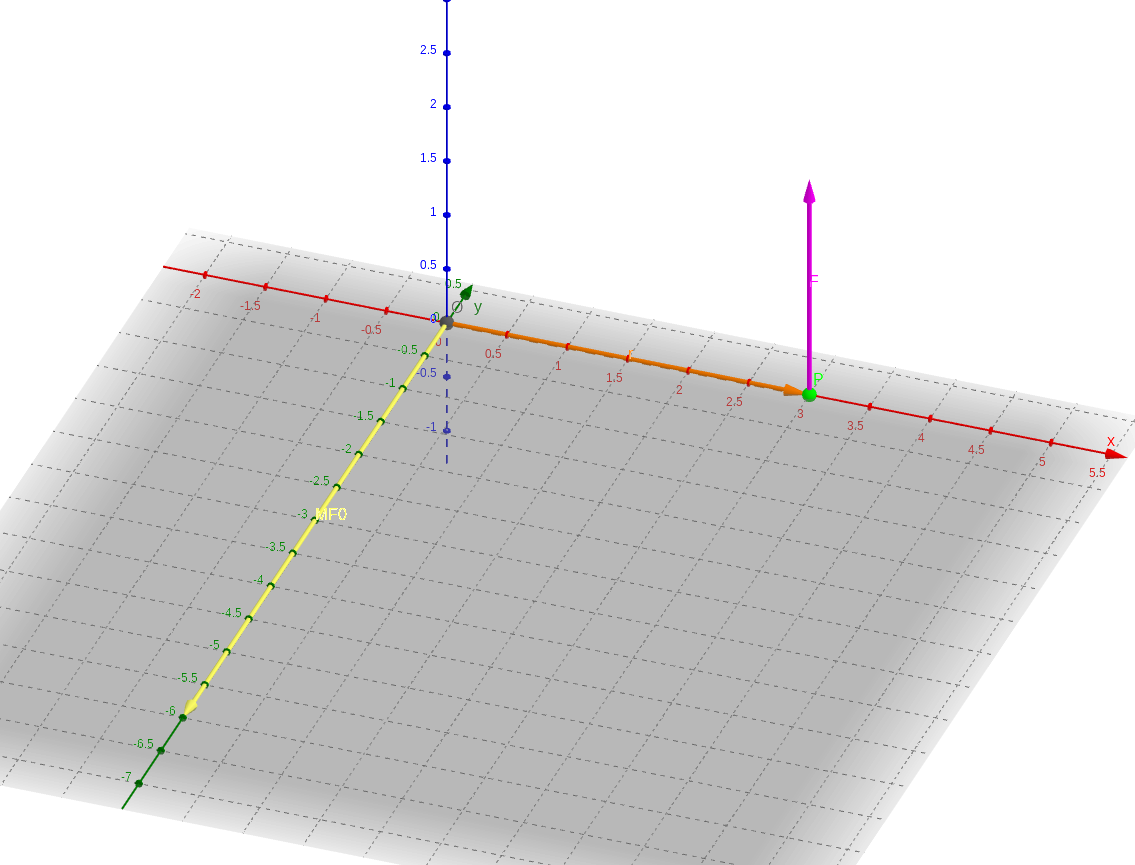
\includegraphics[scale=0.45]{../../common/img/62.01/theory/16-dynamics-torque-01.png}
\label{fig:torque-01}
\end{figure}

En este caso, $\overrightarrow{O} = (0, 0, 0) dm$, $\overrightarrow{P} = (3, 0, 0) dm$ y $\overrightarrow{F} = (0, 0, 2) dN$. Aplicando la definición, $\overrightarrow{M_{F}^{O}} = (0, -6, 0)$. Nótese que el momento es una magnitud vectorial, y es ortogonal a los planos de los vectores $\overrightarrow{r}$ y $\overrightarrow{F}$. Su sentido está dado por la regla de la mano derecha. En este escenario, podría ser que el tornillo estuviera en el origen. Su cabeza estaría en el plano $xz$, y su cuerpo crecería en la dirección positiva del eje $y$. La llave inglesa tendría un largo de 3 decímetros (30 cm) y en su extremo se aplicaría una fuerza de 2 decinewtons en la dirección positiva del eje $z$. Esto daría un momento de $0,06 N m$ (Newton-metro) en la dirección negativa del eje y. Nótese que el momento tiene unidades de fuerza por distancia, que daría unidades de energía, pero nunca se usan Joules o Ergios para el momento para evitar confusiones. Siempre se deja expresado en unidades de fuerza por distancia.

¿Qué interpretación física puede aplicarse al momento? El momento o torque puede entenderse como el equivalente rotacional de las fuerzas lineales, vale decir las que no producen rotación. Si empujamos una caja por su centro, se mueve linealmente, sin rotar; no hay torque. Ahora bien, si la empujamos por un borde, va a rotar además de deslizarse. Va a tener un momento no nulo. De manera más concreta, el torque mide la rotación de un cuerpo alrededor de un eje.

Considérese el módulo del momento:

\begin{equation}
|| \overrightarrow{M_{F}^{O}} || = F r \sin(\alpha(\overrightarrow{r}, \overrightarrow{F}))
\end{equation}

Nótese que al aumentar la magnitud de $r$, aumenta la magnitud del torque: un brazo de palanca más largo produce una mayor rotación. Por ejemplo, una llave inglesa más larga atornilla más rápido. Además, el módulo se maximiza cuando el seno vale 1, o sea cuando alfa vale 90 grados. Ergo, si $\overrightarrow{F} \perp \overrightarrow{r}$, se tiene el máximo torque.

Aunque el momento sea una magnitud vectorial, para ser precisos es en realidad un \textbf{pseudovector}. Al introducir el producto vectorial, el sentido del resultado está dado por la regla de la mano derecha, aunque bien podría estar dado por la mano izquierda. Esta ambigüedad hace que el producto vectorial introduzca cambios de signo espurios al aplicar ciertas transformaciones como espejado alrededor de un eje. Estos problemas no ocurren con vectores puros, por eso se dice que el producto vectorial es un pseudovector. Toda esta cuestión es meramente formalidad matemática y no afecta al mundo de la física.

\subsection{Momento angular}

También conocido como:

\begin{itemize}
\item Momento de la cantidad de movimiento.
\item Momento cinético.
\item Cantidad de movimiento angular.
\end{itemize}

Esta magnitud, como el momento, también es respecto a un punto $\overrightarrow{O}$. Dado un cuerpo de masa $m$ con cierto vector velocidad $\overrightarrow{v}$, su vector cantidad de movimiento es simplemente $\overrightarrow{p} = m \overrightarrow{v}$. Con eso en mente, el momento angular respecto al punto $\overrightarrow{O}$ consiste en:

\begin{equation}
\tcboxmath[colback=orange!25!white,colframe=orange,title=Momento angular de un cuerpo respecto a un punto]{
\quad \quad \quad \overrightarrow{l^O} = (\overrightarrow{P} - \overrightarrow{O}) \times \overrightarrow{p} \quad \quad \quad
}
\end{equation}

No confundir $\overrightarrow{P}$ con $\overrightarrow{p}$. El primero, $\overrightarrow{P}$, es la posición actual del cuerpo, que dicho sea de paso, sigue siendo modelado como partícula. El segundo, $\overrightarrow{p}$, es su vector cantidad de movimiento en el instante de interés, y vale $\overrightarrow{p} = m \overrightarrow{v}$. En cuanto a unidades:

\begin{equation}
[\overrightarrow{l^O}] = [d] [m] [v] = m \mathop{kg} \frac{m}{s}
\end{equation}

Para simplificar, recuérdese que $N = kg \frac{m}{s^2} \Rightarrow N s = kg \frac{m}{s}$. Ergo:

\begin{equation}
[\overrightarrow{l^O}] = N m s
\end{equation}

\subsubsection{Relaciones con momento respecto a un punto}

Derivando miembro a miembro respecto al tiempo la definición de momento angular, y recordando que la regla del producto vale para el producto vectorial, se obtiene:

\begin{equation}
\overrightarrow{l^O} = \overrightarrow{r} \times \overrightarrow{p} \Rightarrow \frac{d\overrightarrow{l^O}}{dt} = \frac{d\overrightarrow{r}}{dt} \times \overrightarrow{p} + \overrightarrow{r} \times \frac{d\overrightarrow{p}}{dt}
\end{equation}

De lo visto en cinemática ya se sabe que $\frac{d\overrightarrow{r}}{dt} = \overrightarrow{v}$, ¿pero qué sería $\frac{d\overrightarrow{p}}{dt}$? Suponiendo que la masa del cuerpo se mantiene constante a lo largo del tiempo:

\begin{equation}
\overrightarrow{p} = m \overrightarrow{v} \Rightarrow \frac{d\overrightarrow{p}}{dt} = m \frac{d\overrightarrow{v}}{dt} = m \overrightarrow{a} = \overrightarrow{F}
\end{equation}

Volviendo a la ecuación inicial:

\begin{equation}
\frac{d\overrightarrow{l^O}}{dt} = \overrightarrow{v} \times \overrightarrow{p} + \overrightarrow{r} \times \overrightarrow{F}
\end{equation}

Ahora bien, nótese que $\overrightarrow{v}$ y $\overrightarrow{p} = m \overrightarrow{v}$ son colineales: el ángulo entre ambos es cero. Por ende, su producto vectorial es nulo. Resulta finalmente:

\begin{equation}
\tcboxmath[colback=orange!25!white,colframe=orange,title=Momento angular y momento]{
\quad \quad \frac{d\overrightarrow{l^O}}{dt} = \overrightarrow{r} \times \overrightarrow{F} = \overrightarrow{M^O_F} \quad \quad
}
\end{equation}

\subsubsection{Relación con impulso}

El momento angular respecto a un punto es entonces la derivada del momento respecto a ese mismo punto. Dado que se tiene dos magnitudes relacionadas mediante la derivada, es de interés integrar miembro a miembro esa relación, y analizar un caso particular.

\begin{equation}
\frac{d\overrightarrow{l^O}}{dt} = \overrightarrow{M^O_F} \Rightarrow \overrightarrow{M^O_F} \mathop{dt} = d\overrightarrow{l^O}
\end{equation}

Integrando miembro a miembro entre un instante $t_0$ y un instante $t_f$, y aplicando la definición de momento:

\begin{equation}
\int_{t_0}^{t_f} (\overrightarrow{r} \times \overrightarrow{F}) dt = \int_{\overrightarrow{l^O_0}}^{\overrightarrow{l^O_f}} d\overrightarrow{l^O}
\end{equation}

El lado derecho de la igualdad es simplemente la variación de momento angular, que se denotará $\Delta\overrightarrow{l^O} = \overrightarrow{l^O_f} - \overrightarrow{l^O_0}$.

Llegado este punto, es donde se analizará un caso particular: las \textbf{fuerzas impulsivas}. Recuérdese que una fuerza impulsiva es una fuerza relativamente intensa que se aplica a un cuerpo durante un instante muy corto de tiempo. Se asume entonces que $\Delta t \rightarrow 0$, y que $\overrightarrow{r}$ permanece constante durante ese intervalo infinitesimal. Con estas hipótesis:

\begin{equation}
\overrightarrow{r} \times \int_{t_0}^{t_f} \overrightarrow{F} dt = \Delta \overrightarrow{l^O}
\end{equation}

La integral de la fuerza respecto al tiempo en un intervalo infinitesimal es justamente la definición de impulso:

\begin{equation}
\tcboxmath[colback=orange!25!white,colframe=orange,title=Impulso]{
\overrightarrow{J} = \lim_{\Delta t \rightarrow 0} \int_{t_0}^{t_f} \overrightarrow{F} dt
}
\end{equation}

De esta manera, para el caso de fuerzas impulsivas, se tiene:

\begin{equation}
\tcboxmath[colback=orange!25!white,colframe=orange,title=Momento angular e impulso]{
\quad \quad \quad \overrightarrow{r} \times \overrightarrow{J} = \Delta \overrightarrow{l^O} \quad \quad \quad
}
\end{equation}

\subsubsection{Conservación de momento angular}

Considérese un escenario donde actuén fuerzas impulsivas, y se tenga $\Delta \overrightarrow{l^O} = 0$. Vale decir, el momento angular es constante. Esto puede desdoblarse en los siguientes escenarios:

\begin{itemize}
\item $\overrightarrow{r} \parallel \overrightarrow{J} $. Si son paralelos, el producto vectorial es nulo.
\item $\sum \overrightarrow{J} = 0$
\begin{itemize}
\item $\sum \overrightarrow{F} = 0$
\item $\overrightarrow{F} = \overrightarrow{cte}$
\item No hay fuerzas.
\end{itemize}
\item $\overrightarrow{r} = 0$. En este caso, el impulso pasa por el eje de momentos.
\end{itemize}

\subsubsection{Conservación de la cantidad de movimiento}

Nuevamente en un escenario con fuerzas impulsivas, recuérdese la relación entre impulso y cantidad de movimiento:

\begin{equation}
\tcboxmath[colback=orange!25!white,colframe=orange,title=Impulso y $\overrightarrow{p}$]{
\quad \quad \sum \overrightarrow{J} = \Delta \overrightarrow{p} \quad \quad
}
\end{equation}

Entonces, si $\Delta \overrightarrow{p} = 0 \Rightarrow \sum \overrightarrow{J} = 0$, lo cual corresponde a los mismos tres subescenarios de la sección anterior:

\begin{itemize}
\item $\sum \overrightarrow{F} = 0$
\item $\overrightarrow{F} = \overrightarrow{cte}$
\item No hay fuerzas.
\end{itemize}

\subsection{Sistema de partículas}

Hasta ahora, se han modelado todos los cuerpos como partículas puntuales, vale decir, toda la masa se consideraba concentrada en un punto. Como generalización de este concepto, se considerará ahora un modelo para analizar un conjunto de partículas. En un instante determinado, se tiene una configuración específica en cuanto a posición, velocidad y aceleración de cada partícula. Para analizar el conjunto como si fuera una sola partícula, se introduce el concepto de \textbf{centro de masa (CM)}. Con ello, será posible reutilizar todas las técnicas ya vistas para una sola partícula.

Si $\overrightarrow{r}_i$, $\overrightarrow{v}_i$ y $\overrightarrow{a}_i$ son la posición, velocidad y aceleración instantáneas de la i-ésima partícula de un total de $N$ partículas, dichas magnitudes para el centro de masa estarán dadas por:

\begin{equation}
\tcboxmath[colback=orange!25!white,colframe=orange,title=Posición del CM]{
\overrightarrow{r_{\text{CM}}} = \frac{\sum\limits_{i=1}^N m_i \overrightarrow{r_i}}{\sum\limits_{i=1}^N m_i}
}
\end{equation}

\begin{equation}
\tcboxmath[colback=orange!25!white,colframe=orange,title=Velocidad del CM]{
\quad \overrightarrow{v_{\text{CM}}} = \frac{\sum\limits_{i=1}^N m_i \overrightarrow{v_i}}{\sum\limits_{i=1}^N m_i} \quad
}
\end{equation}

\begin{equation}
\tcboxmath[colback=orange!25!white,colframe=orange,title=Aceleración del CM]{
\quad \overrightarrow{a_{\text{CM}}} = \frac{\sum\limits_{i=1}^N m_i \overrightarrow{a_i}}{\sum\limits_{i=1}^N m_i} \quad
}
\end{equation}

Nótese que estas expresiones valen coordenada a coordenada. Vale decir, si se desea calcular la coordenada $y$ de la posición del centro de masa, se hace el mismo promedio ponderado sobre la coordenada $y$ de todas las partículas. Y lo mismo vale para velocidad y aceleración.

En cuanto a la cantidad de movimiento, es posible demostrar que para este modelo, la cantidad de movimiento del CM es la suma de la cantidad de movimiento de todas las partículas. Ergo, si se define $M_T = \sum_{i=1}^N m_i$:

\begin{equation}
\tcboxmath[colback=orange!25!white,colframe=orange,title=Cantidad de movimiento del CM]{
\quad \quad \overrightarrow{p_{\text{CM}}} = M_T \overrightarrow{v_\text{CM}} = \sum_{i=1}^N \overrightarrow{p_i} \quad \quad
}
\end{equation}

\subsubsection{Segunda ley de Newton para SP}

Para reformular la segunda ley de Newton en el contexto de sistemas de partículas (SPs), es necesario introducir el concepto de \textbf{fuerzas internas y externas}. Dado un sistema de partículas, las fuerzas surgidas de interacciones entre las partículas se consideran internas, y todas las demás se consideran externas. Si se aplica la segunda ley al SP:

\begin{equation}
\sum \overrightarrow{F} = m \overrightarrow{a}
\end{equation}

En el lado izquierdo de la igualdad, es posible desdoblar las fuerzas en internas y externas. En el lado derecho, la masa del sistema es $M_T$, y la aceleración es $\overrightarrow{a_{\text{CM}}}$. 

\begin{equation}
\sum \overrightarrow{F_{\text{int}}} + \sum \overrightarrow{F_{\text{ext}}} = M_T \overrightarrow{a_{\text{CM}}}
\end{equation}

Ahora bien, por la 3ra ley de Newton, dado que las fuerzas internas son pares acción-reacción, se cancelan entre sí y su suma es cero. Por ende, resulta:

\begin{equation}
\tcboxmath[colback=orange!25!white,colframe=orange,title=2da ley de Newton para SP]{
\quad \quad \sum \overrightarrow{F_{\text{ext}}} = M_T \overrightarrow{a_{\text{CM}}} \quad \quad
}
\end{equation}

Para el caso particular en que $\sum \overrightarrow{F_{\text{ext}}} = 0$, se conserva la cantidad de movimiento del centro de masa: 

\begin{equation}
\sum \overrightarrow{F_{\text{ext}}} = 0 \Rightarrow \overrightarrow{p_{\text{CM}}} = \text{cte}
\end{equation}

Si se ubica el sistema de referencia en el CM, resulta:

\begin{equation}
0 = \sum_{i=1}^N m_i (\overrightarrow{v_i} - \overrightarrow{v_{\text{CM}}})
\end{equation}

\subsubsection{Trabajo y energía en SP}

Por definición, la energía cinética total del sistema está dada por:

\begin{equation}
\tcboxmath[colback=orange!25!white,colframe=orange,title=Energía cinética total de un SP]{
\quad \qquad E_c = \frac{1}{2} \sum_{i=1}^N m_i ||\overrightarrow{v_i}||^2 \qquad \quad
}
\end{equation}

Y la energía potencial gravitatoria:

\begin{equation}
\tcboxmath[colback=orange!25!white,colframe=orange,title=$E_{\text{pg}}$ total de un SP]{
\quad E_{\text{pg}} = M_T g h_{\text{CM}} \quad
}
\end{equation}

En esta expresión, la altura del centro de masa, $h_{\text{CM}}\textbf{•}$, estará dada por la coordenada de su vector posición que represente la distancia al cero de referencia.

Para vincular dos instantes de tiempo, es posible aplicar:

\begin{equation}
\sum_{i=1}^N W_i = \Delta E_c
\end{equation}

\begin{equation}
\sum_{i=1}^N W_{\mathop{f\cancel{c}}} = \Delta E_m, E_m = E_c + E_{\text{pg}}
\end{equation}

Es esencial tener en cuenta que en estas expresiones, se incluye el trabajor realizado por las fuerzas internas.

Otra magnitud que puede resultar de interés es la energía cinética respecto al CM, la cual se define como:

\begin{equation}
\tcboxmath[colback=orange!25!white,colframe=orange,title=$E_c$ respecto a CM]{
\quad E_{\text{C-CM}} = E_c - \frac{1}{2} M_T ||\overrightarrow{v_{\text{CM}}}||^2 \quad
}
\end{equation}

El momento angular del CM es la suma de momento angulares respecto al CM:

\begin{equation}
\tcboxmath[colback=orange!25!white,colframe=orange,title=Momento angular del CM]{
\quad \qquad \overrightarrow{l^{\text{CM}}} = \sum_{i=1}^N \overrightarrow{l_i^{\text{CM}}} \qquad \quad
}
\end{equation}

Esto implica que la relación entre momento y momento angular es:

\begin{equation}
\tcboxmath[colback=orange!25!white,colframe=orange,title=Momento y momento angular del CM]{
\qquad \qquad \sum_{i=1}^N \overrightarrow{M_{\text{ext}}^{\text{CM}}} = \frac{d\overrightarrow{l^{\text{CM}}_i}}{\mathop{dt}} \qquad \qquad
}
\end{equation}

Para escenarios con fuerzas impulsivas, puede demostrarse que:

\begin{equation}
\tcboxmath[colback=orange!25!white,colframe=orange,title=Impulsos y SP]{
\sum_{i=1}^N \overrightarrow{J_{\text{ext}}} = \Delta \overrightarrow{p_{\text{CM}}}
}
\end{equation}

\subsubsection{Choques mecánicos}

Para simplificar el planteo, se considera que el intervalo de choque es un infinitésimo. Más específicamente, se define como intervalo de choque el lapso de tiempo transcurrido desde que los cuerpos empiezan a juntarse hasta que los cuerpos empiezan a separarse. Esto último tendrá una salvedad en el caso particular del choque plástico, como se verá más adelante. Por otro lado, las fuerzas externas que puedan llegar a actuar se consideran despreciables en comparación con las fuerzas impulsivas generadas por el choque. Dado que dichas fuerzas son internas al sistema, su suma es nula. Por ende, la sumatoria total de fuerzas es nula, y se conserva la cantidad de movimiento. Resumiendo, para todo choque mecánico, se cumplirá:

\begin{itemize}
\item $\Delta t \rightarrow 0$
\item $\Delta \overrightarrow{p_{\text{CM}}} = 0$
\end{itemize}

Antes de analizar los diferentes tipos de choque mecánico, es de utilidad introducir el \textbf{coeficiente de restitución}, definido como:

\begin{equation}
\tcboxmath[colback=orange!25!white,colframe=orange,title=Coeficiente de restitución]{
e = -\frac{P_I(\overrightarrow{v_{f2}} - \overrightarrow{v_{f1}})}{P_I(\overrightarrow{v_{02}} - \overrightarrow{v_{01}})}
}
\end{equation}

En esta expresión, $\overrightarrow{v_{f2}}$ es la velocidad final del cuerpo 2. Por velocidad final, se entienda la que adquiere inmediatamente después del choque. Análogamente, la velocidad inicial de cada cuerpo es la medida inmediatamente antes del choque. Esto implica naturalmente que se está considerando siempre un choque entre 2 cuerpos, y que uno debe rotularse como cuerpo 1 y otro como cuerpo 2.

En cuanto a la expresión $P_I$, es un operador que recibe un vector velocidad y devuelve un escalar que representa la proyección de dicho vector en la dirección del impacto. La pregunta obvia que surge es cuál es la dirección del impacto. De manera general, al chocar dos cuerpos en 3 dimensiones, es posible determinar una superficie de impacto, que en el caso de un modelo de partículas, será un plano de impacto. La dirección de impacto estará entonces dada por la normal de dicho plano; el sentido elegido como positivo es irrelevante, en tanto se use consistentemente.

\textbf{Tipos de choque mecánico}:

\begin{itemize}
\item \textbf{Perfectamente elástico}: Los cuerpos no se deforman, y se conserva la energía cinética. Obviamente este es un caso idealizado que jamás se observa en la realidad, pero en muchos casos se da de manera aproximada. Por ejemplo, un choque entre bolas de billar es algo bastante cercano a un choque totalmente elástico. Este caso corresponde a $e = 1$.
\item \textbf{Inelástico}: Hay cierto grado de deformación en ambos cuerpos. Casi todos los choques reales caen en este rango, que corresponde a $0 < e < 1$.
\item \textbf{Plástico/perfectamente inelástico}: Luego del choque, los cuerpos permanecen unidos, y se mueven con la misma velocidad $\overrightarrow{v_f}$. En este caso, $e = 0$. Por ejemplo, un camión chocando un mosquito.
\item \textbf{Explosivo}: Este choque ocurre cuando se gana energía cinética. Esto puede ocurrir, por ejemplo, si un cuerpo tiene energía potencial que se convierte en cinética. Por ejemplo, si un cuerpo lleva un resorte y éste se activa durante el choque. En casos así, $e > 1$.
\item \textbf{Con penetración}: Un cuerpo se incrusta en el otro y lo atraviesa. Es en estos casos donde más energía cinética se pierde, y el cuerpo atravesado sufre ese impacto. Estos casos corresponden a $e < 0$.
\end{itemize}

\end{document}